\documentclass[aspectratio=169]{beamer} %[aspectratio=169]
\usetheme{Boadilla}
\usecolortheme{seahorse}

\usepackage{parskip}

% հայկական և լատինական տառատեսակի կարգավորում
\usepackage{fontspec}
% \usepackage{polyglossia}
% \setdefaultlanguage{armenian}
% \newfontfamily\armenianfont{GHEA Mariam}
\setmainfont{DejaVu Serif}
\setsansfont{DejaVu Sans}
\setmonofont{DejaVu Sans Mono}
% \setmainfont{/home/srohund/Documents/1991/Arti Regular.otf}

% մաթեմի տառատեսակ
\usepackage{unicode-math}
% Set the math font to Fira Math

% Գույների համար
\usepackage{xcolor}
\definecolor{seahorseblue}{RGB}{0, 102, 204}
\definecolor{seahorsered}{RGB}{204, 0, 0}
\definecolor{seahorsegreen}{RGB}{0, 153, 0}
\definecolor{seahorseyellow}{RGB}{255, 204, 0}

\definecolor{seahorseblue2}{RGB}{0, 105, 148}
\definecolor{seahorsegreen2}{RGB}{0, 128, 71}
\definecolor{seahorsered2}{RGB}{217, 0, 27}
\definecolor{seahorseorange2}{RGB}{255, 123, 0}
\definecolor{seahorsegray2}{RGB}{92, 92, 92}
\definecolor{seahorsepink2}{RGB}{214, 0, 96}
\definecolor{seahorseyellow2}{RGB}{255, 201, 0}

% հղումների համար
\usepackage{hyperref}
\hypersetup{
	colorlinks=true,
	linkcolor=seahorsered,
	urlcolor=seahorseblue,
	citecolor=seahorsegreen,
}

% պատկերներ
\usepackage{graphicx}
\graphicspath{ {./images/} } % \includegraphics


% հիմնական տվյալներ
\title[մաթ․ անալիզ - դաս 1]{1991 ստորաբաժանման դիմորդների նախապատրաստական դասընթաց}
\subtitle{Մաթեմաթիկական անալիզի ներածություն, դաս 1}
\author[Առաքելյան Ա․]{
    \href{mailto:aram.arakeljan@gmail.com}{Առաքելյան Արամ}
}
\institute{\href{https://1991.mil.am/}{«1991» ակադեմիա}}

\date{2023թ դեկտեմբեր}
\begin{document}
    % գլխարկ
    \begin{frame}
        \titlepage
	% \maketitle
    \end{frame}
%     %%%%%%%%%%%%%%% դաս 1 %%%%%%%%%%%%%%%
     \section{դաս 1}
%     %%%%%%%       մոտիվացիա       %%%%%%%
    \subsection{մոտիվացիա}
    % \begin{frame}
    %     \frametitle{Ինչու՞ մաթեմատիկական անալիզ}
    %     % TODO
    %     \centering{Շուտով․․․}
    % \end{frame}
    % \begin{frame}
    %     \frametitle{Դասընթացի կառուցվածքը}
    %     % TODO
    %     \centering{Շուտով․․․}
    % \end{frame}
    %%%%%%%   բովանդականություն   %%%%%%%
    \begin{frame}
    \frametitle{Բովանդականություն}
    \begin{block}{}
        Անընդհատություն\\
        «Աքիլլեսն ու կրիան»\\
        Սահմանային անցում\\
    \end{block}
    \begin{block}{}
        Հաջորդականություն\\
        \begin{itemize}
            \item Բնական թվեր
        \end{itemize}
    \end{block}
    \begin{block}{}
        Ֆունդամենտալ հաջորդականություն\\
        \begin{itemize}
            \item Հաջորդականություն սահմանափակությունը
            \item Հանրահաշվական գործողություններ
        \end{itemize}
    \end{block}
    
    
    \end{frame}
    %%%%%%%    անընդհատություն    %%%%%%%
    \subsection{անընդհատություն}
    \begin{frame}
        \frametitle{Անընդհատություն}
        Հայկը իր \only<1-4, 16-> {$50000$}	\only<5-15>{$k$} դրամը ավանդ է ներդնում բանկում \only<1-4, 16-> {$15\%$} \only<5-15> {$p$} տարեկան տոկոսադրույքով։\\
        \only<3->{
            \begin{alertblock}{Հարց}
                Հնարավո՞ր է, որ գումարը \only<4>\alert{անընդհատ} աճի։
	    \end{alertblock}
        }
        \only<2, 3>{
            \centering{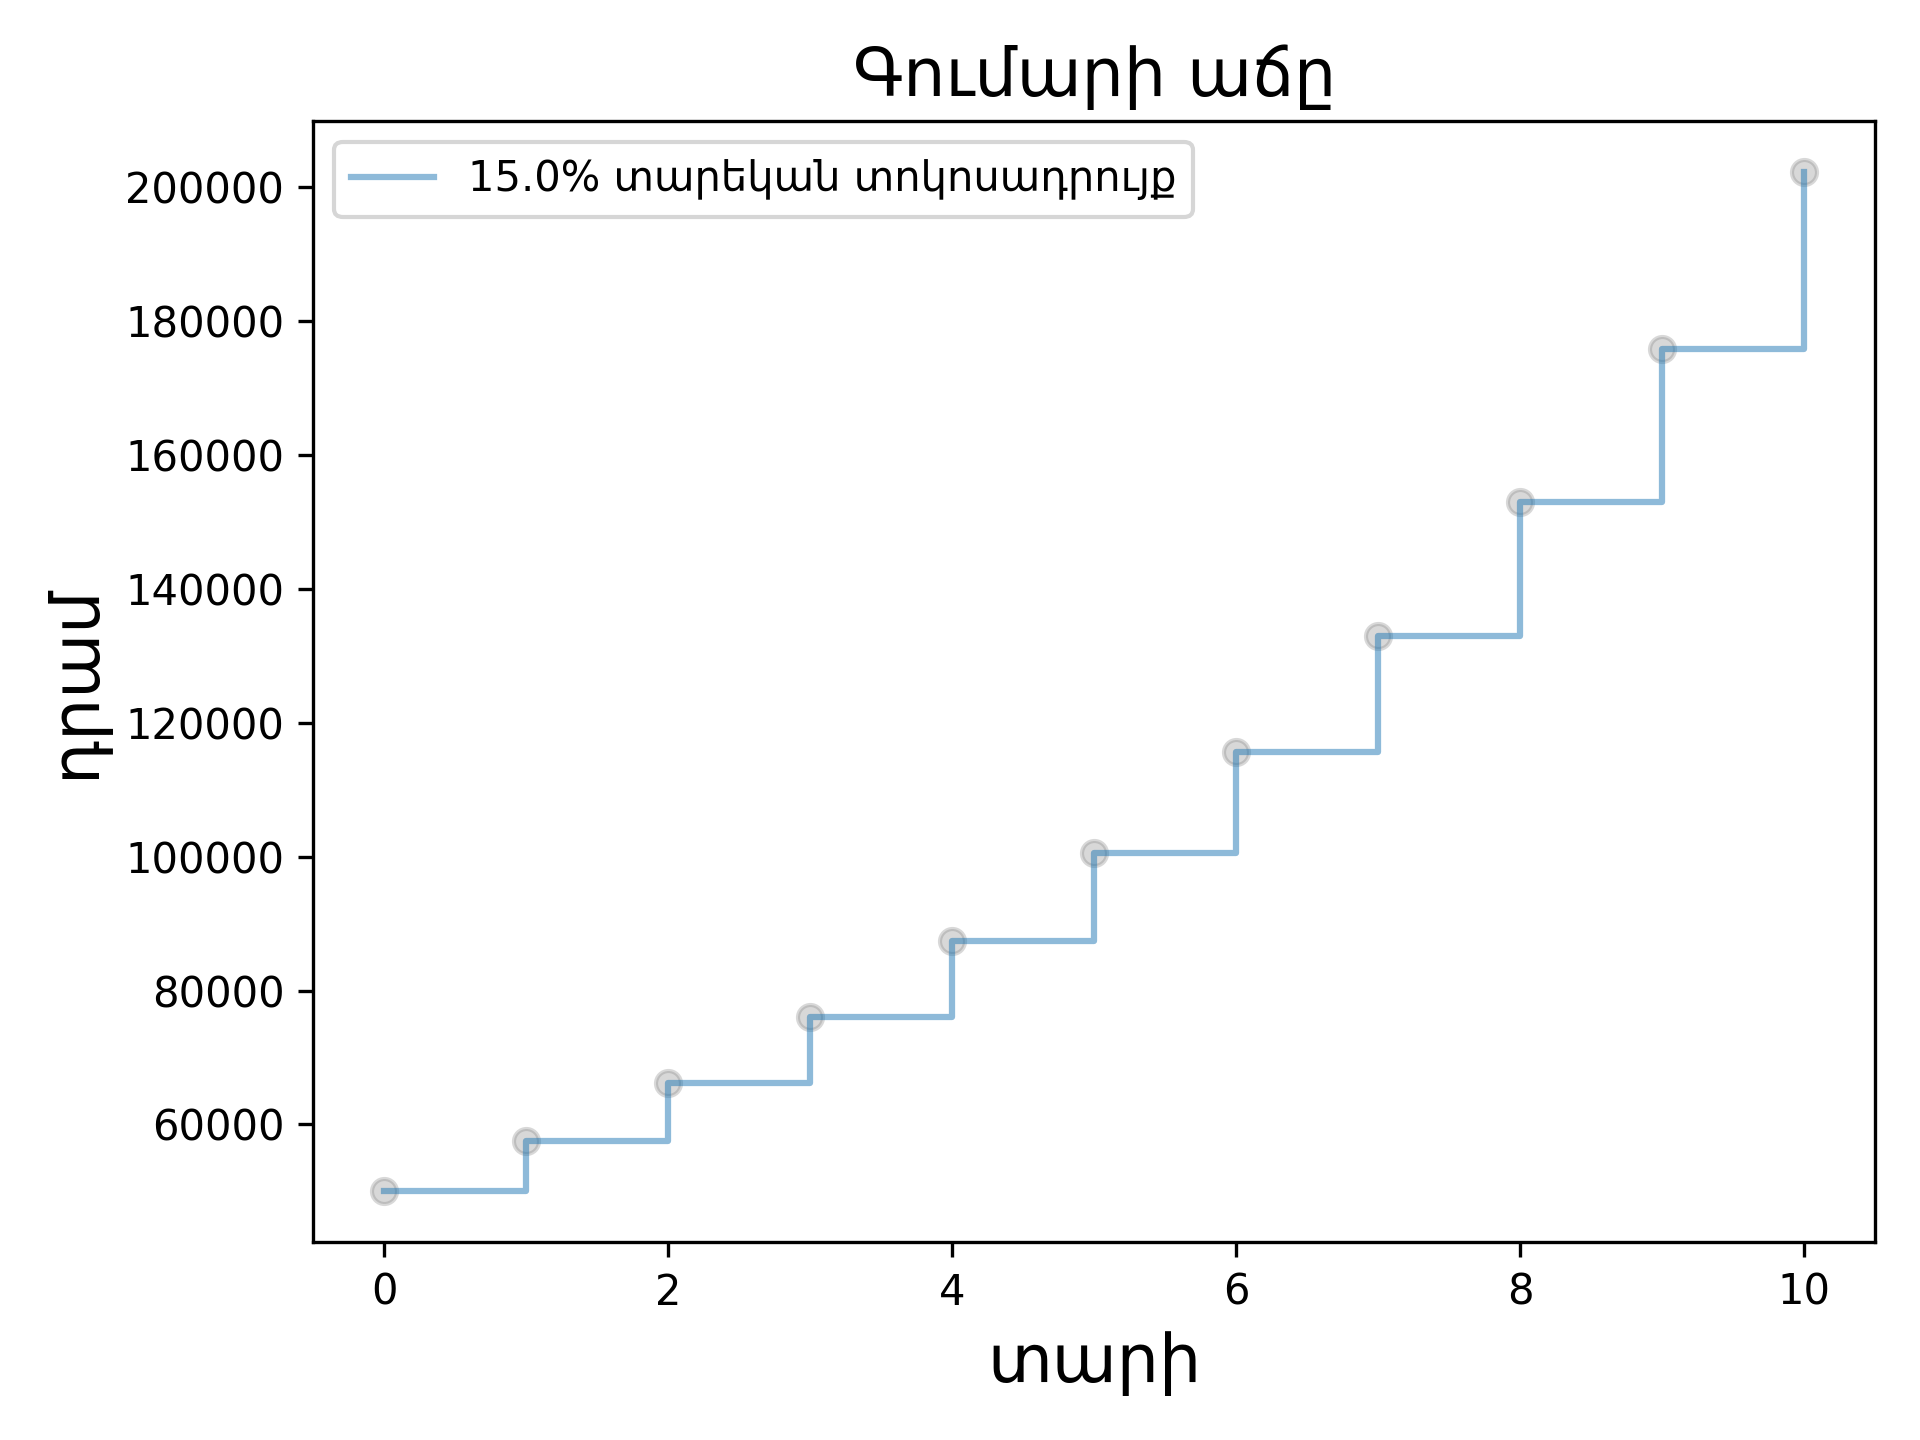
\includegraphics[width=0.4\textwidth]{1_0x100.png}}
        }
	    \only<4>{
	    	\centering{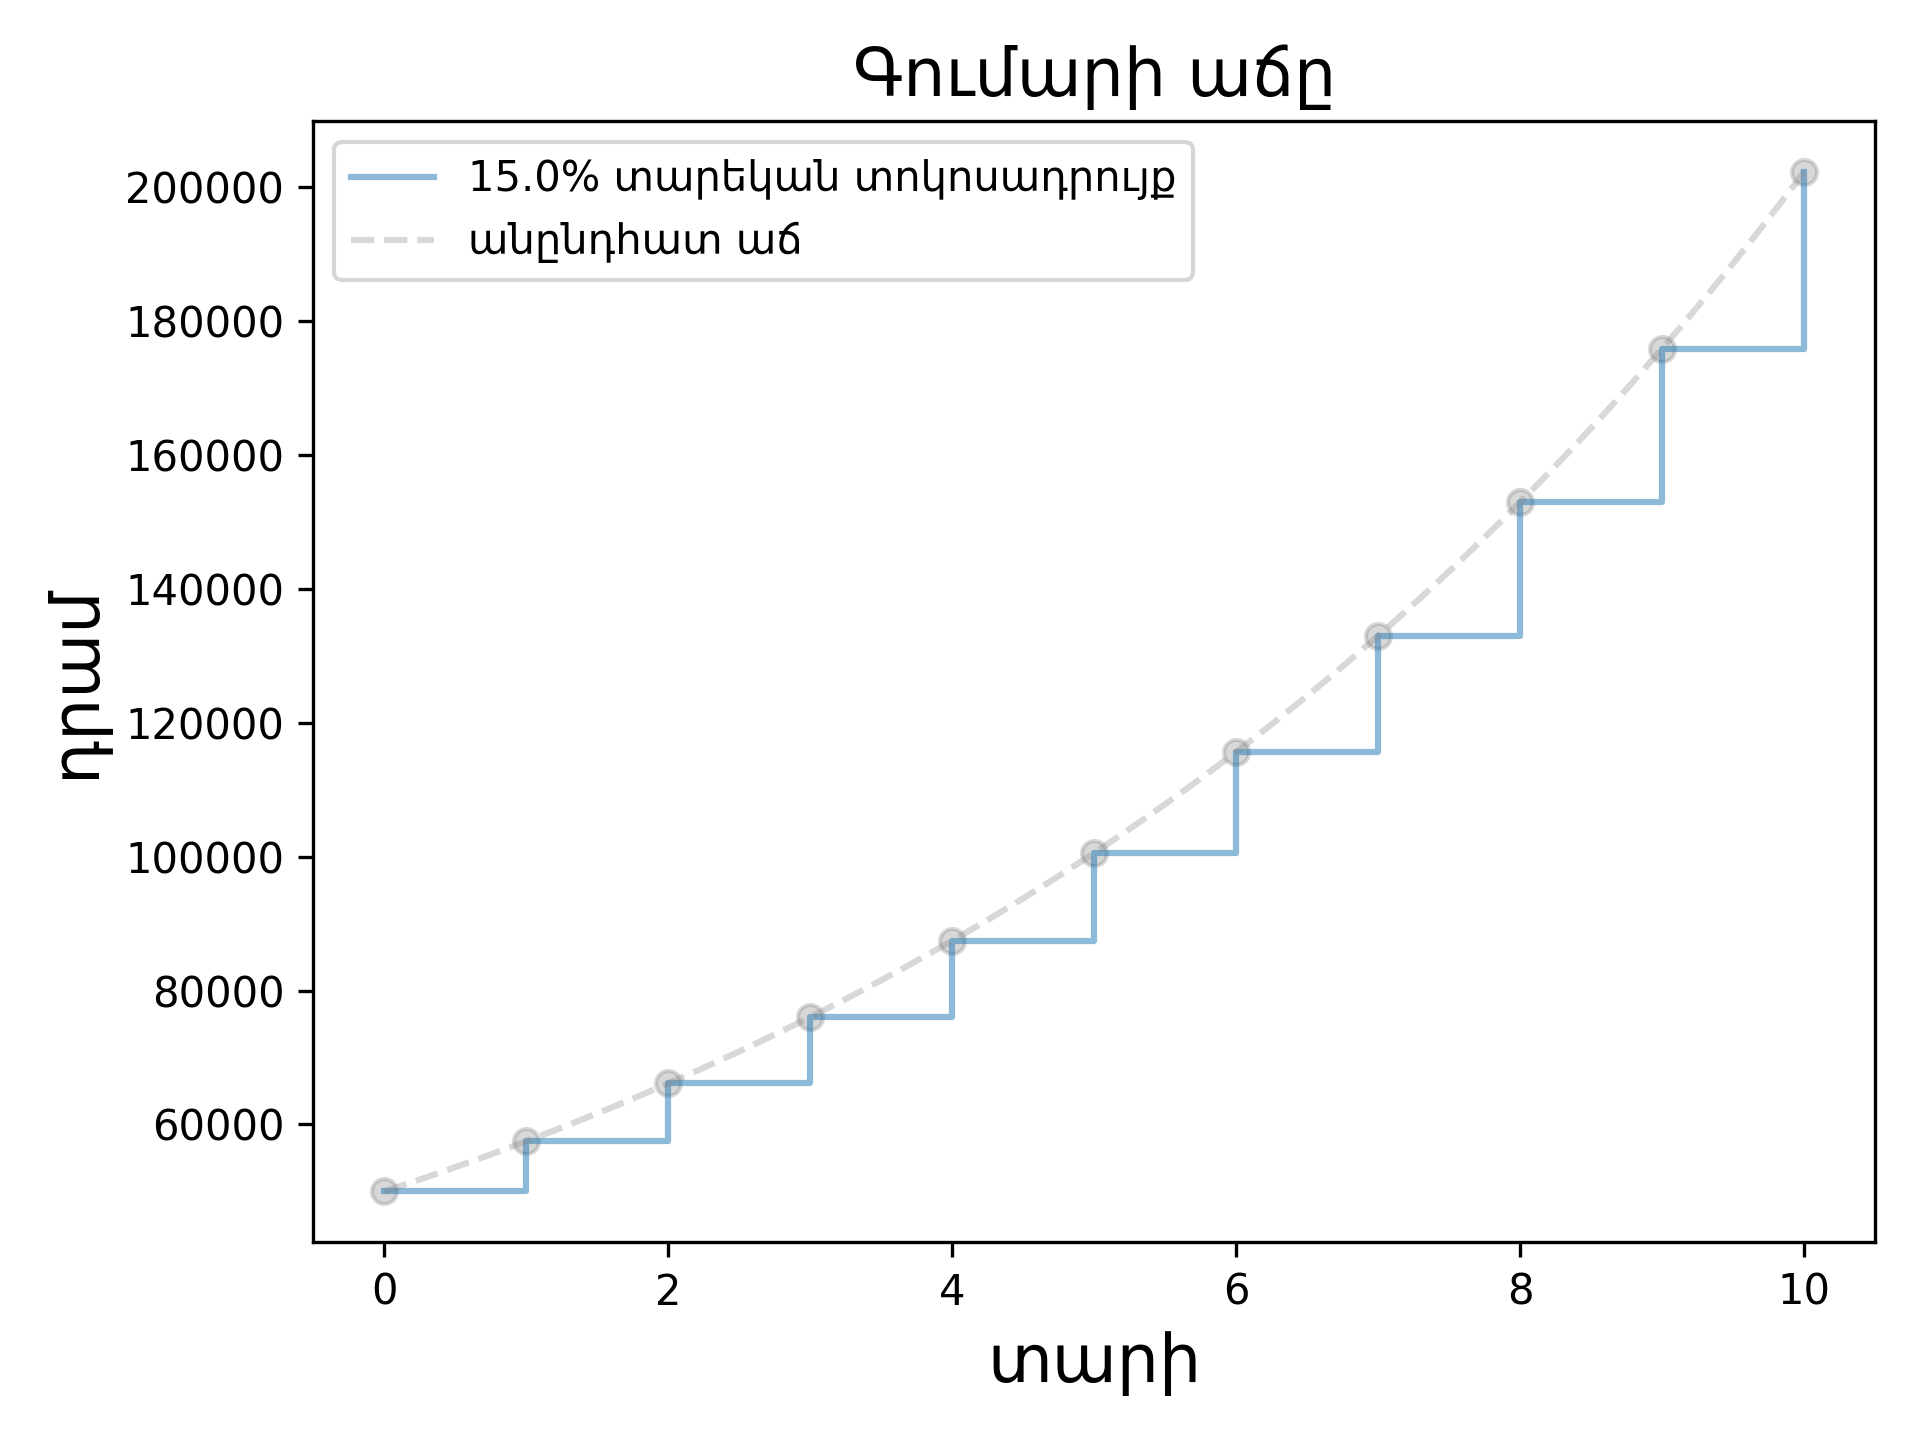
\includegraphics[width=0.4\textwidth]{1_0x100_c.png}}
	    }
        \only<5-15>{\only<5>\alert{$x_n$} - $n$-րդ տարում Հայկի ունեցած գումարը}
        \only<6-10>{
        	\begin{align*}
        		\only<6->{x_{n+1} & = \left(1+\frac{p}{100}\right)x_n\\}
        		\only<7-8>{& = \left(1+\frac{p}{100}\right)^2x_{n-1}\\}
        		\only<8-8>{& = \left(1+\frac{p}{100}\right)^3x_{n-2}\\}
        		\only<9->{& \vdots \\ & = \left(1+\frac{p}{100}\right)^{n+1}x_{0} \only<10->{ = k\left(1+\frac{p}{100}\right)^{n+1}}}
        	\end{align*}
        }
        \only<11-15>{\[x_n = k\left(1+\frac{p}{100}\right)^n\]}
        \only<12-15>{եթե Յուրաքանչյուր կես տարին մեկ գումարը աճի, ապա՝}
        \only<13-15>{
        	\only<13>{\[\tilde{x}_m = k \left(\sqrt[2]{1+\frac{p}{100}}\right)^m\]}
            \only<14>{
                \\երբ $m = 2n$
                \[\tilde{x}_m = k \left(\sqrt[2]{1+\frac{p}{100}}\right)^m = k \left(\sqrt[2]{1+\frac{p}{100}}\right)^{2n}\]
            }
            \only<15>{
                \\երբ $m = 2n$
                \[\tilde{x}_m = k \left(\sqrt[2]{1+\frac{p}{100}}\right)^m = k \left(1+\frac{p}{100}\right)^{n} = x_n\]
            }
        	որտեղ \alert<13>{$m$}-ը անսած կես տարիների քանակն է
    	}
    	\only<16>{
    		\centering{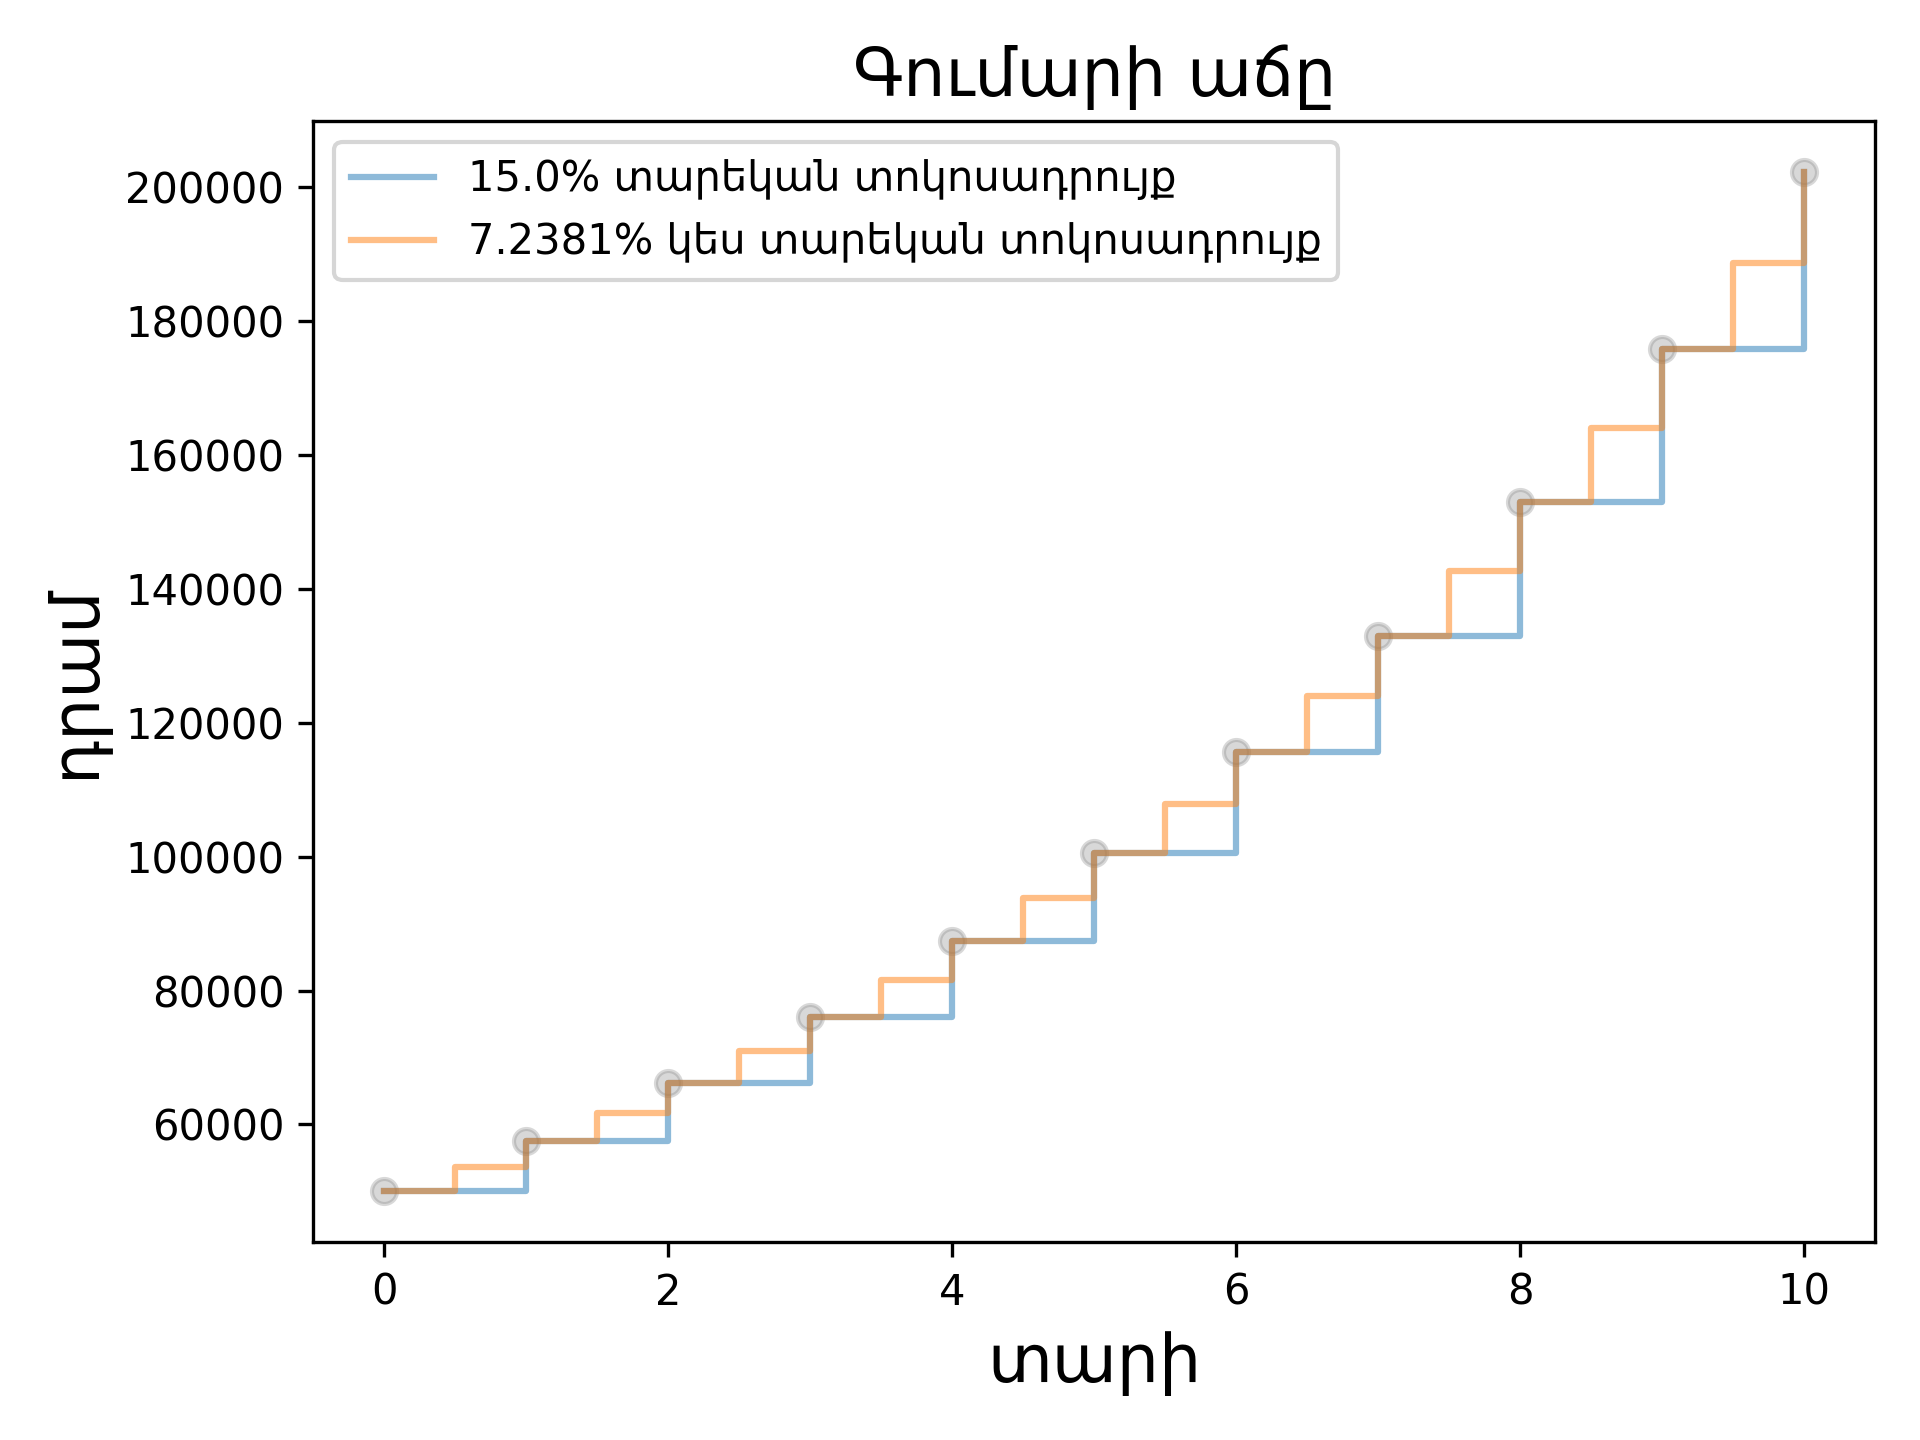
\includegraphics[width=0.4\textwidth]{1_2_0x100.png}}
    	}
    	\only<17-18>{
    		$1$ տարվա ընթացքում, $m$ անգամ գումարի աճելու դեպքում, տարվա $t$-րդ պահին գումարը լինում է՝
    		\only<18->{\[50000 \left(\sqrt[m]{1+\frac{15}{100}}\right)^{[mt]},\] որտեղ $[x]$-ը $x$ թվի ամբողջ մասն է։}
    		% \includegraphics[width=0.2\textwidth]{1_2_12_40x50_c.png}
    	}
        \only<19>{
	    	\centering{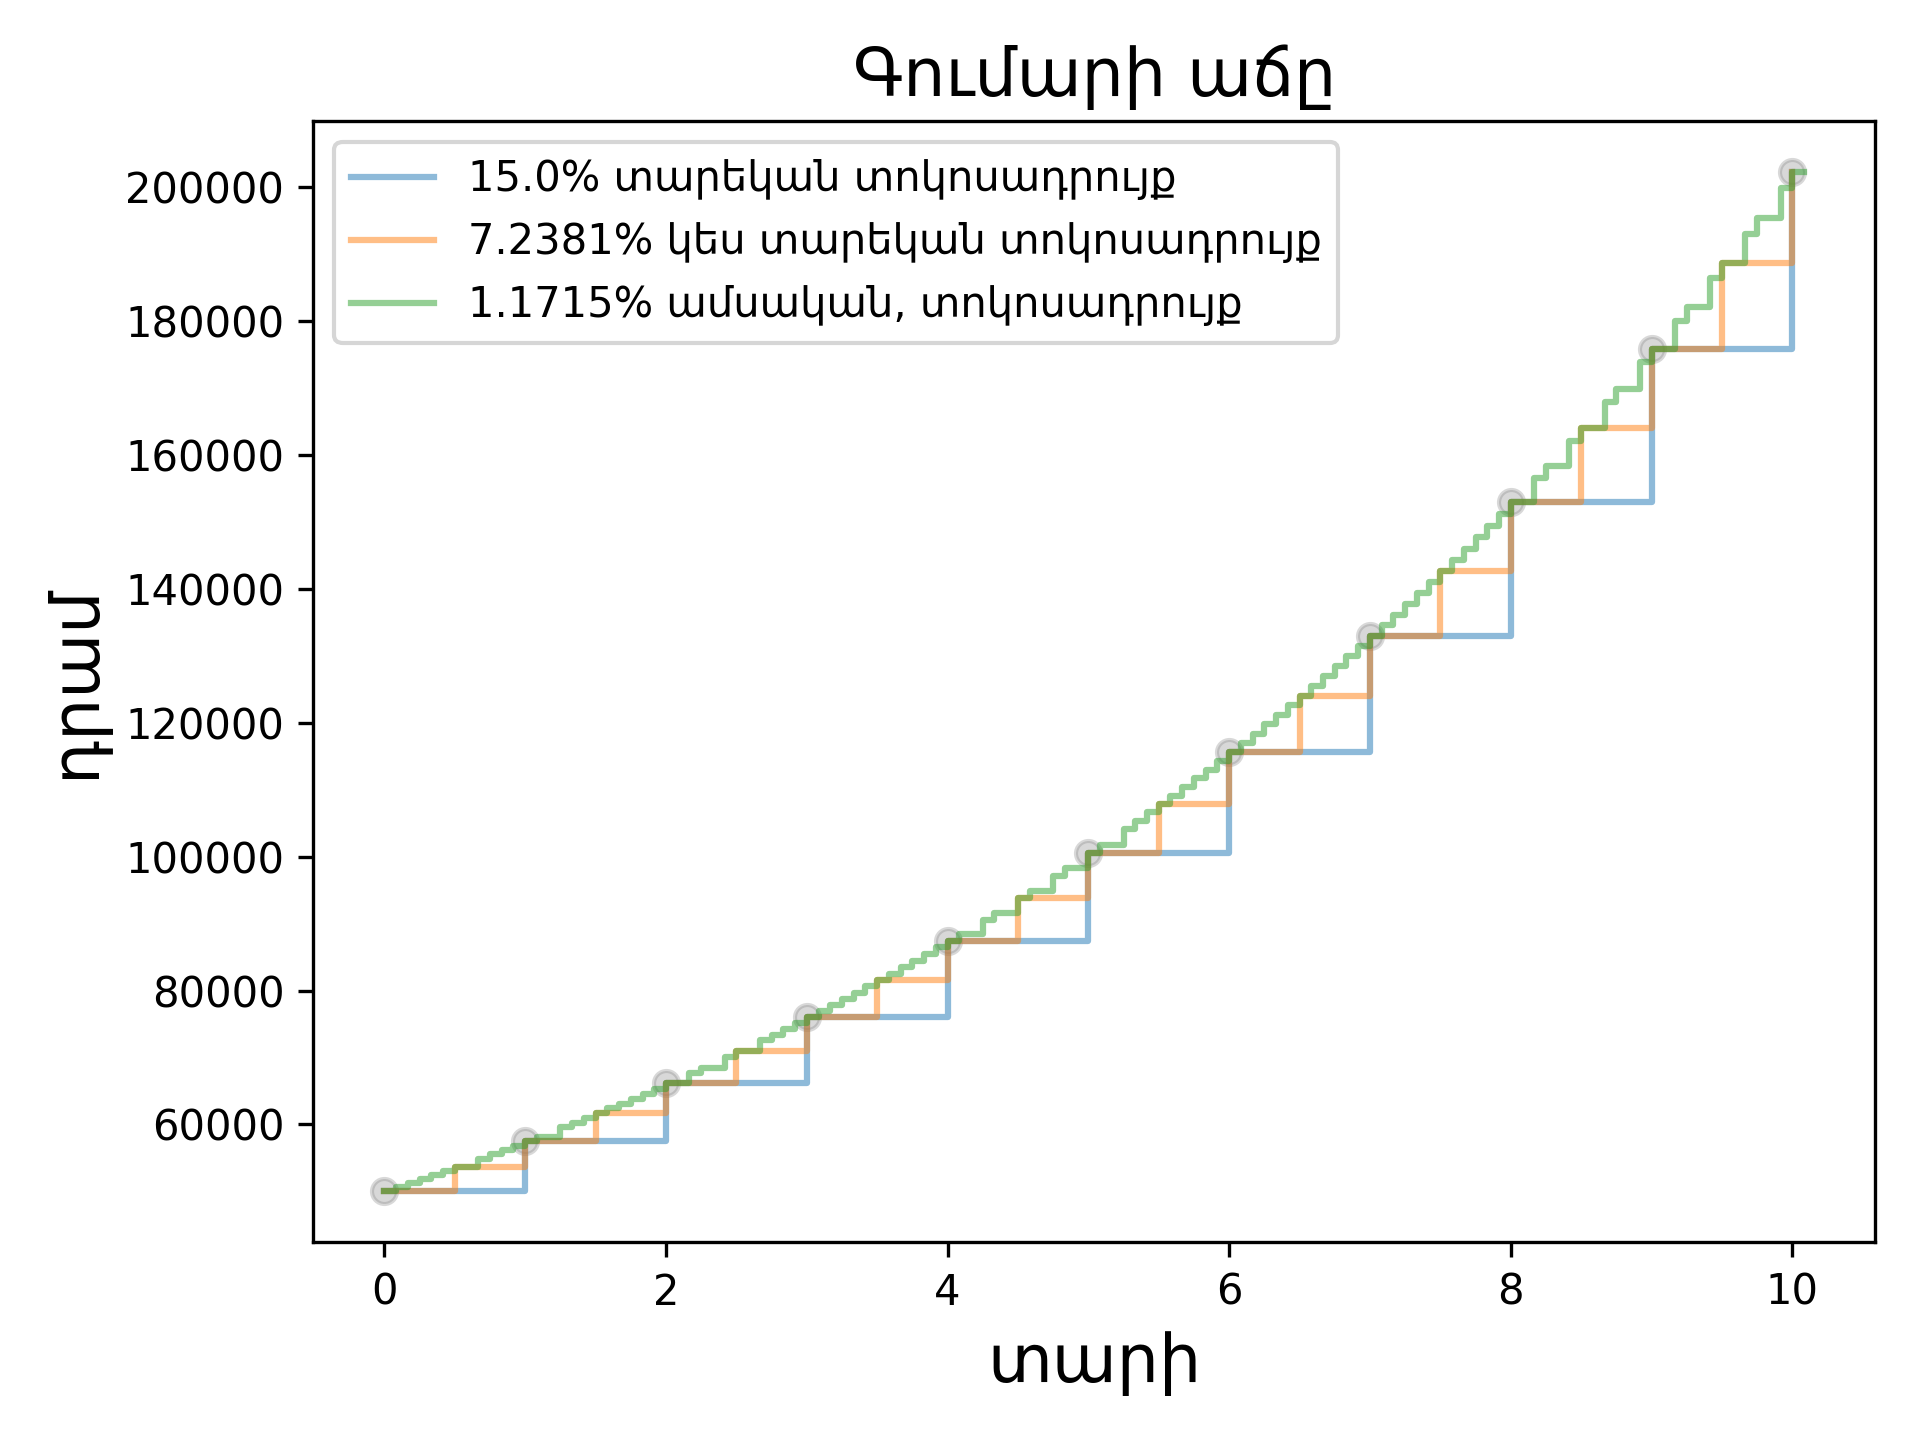
\includegraphics[width=0.4\textwidth]{1_2_12_0x100.png}}
	    }
	    \only<20>{
	    	\centering{
	    		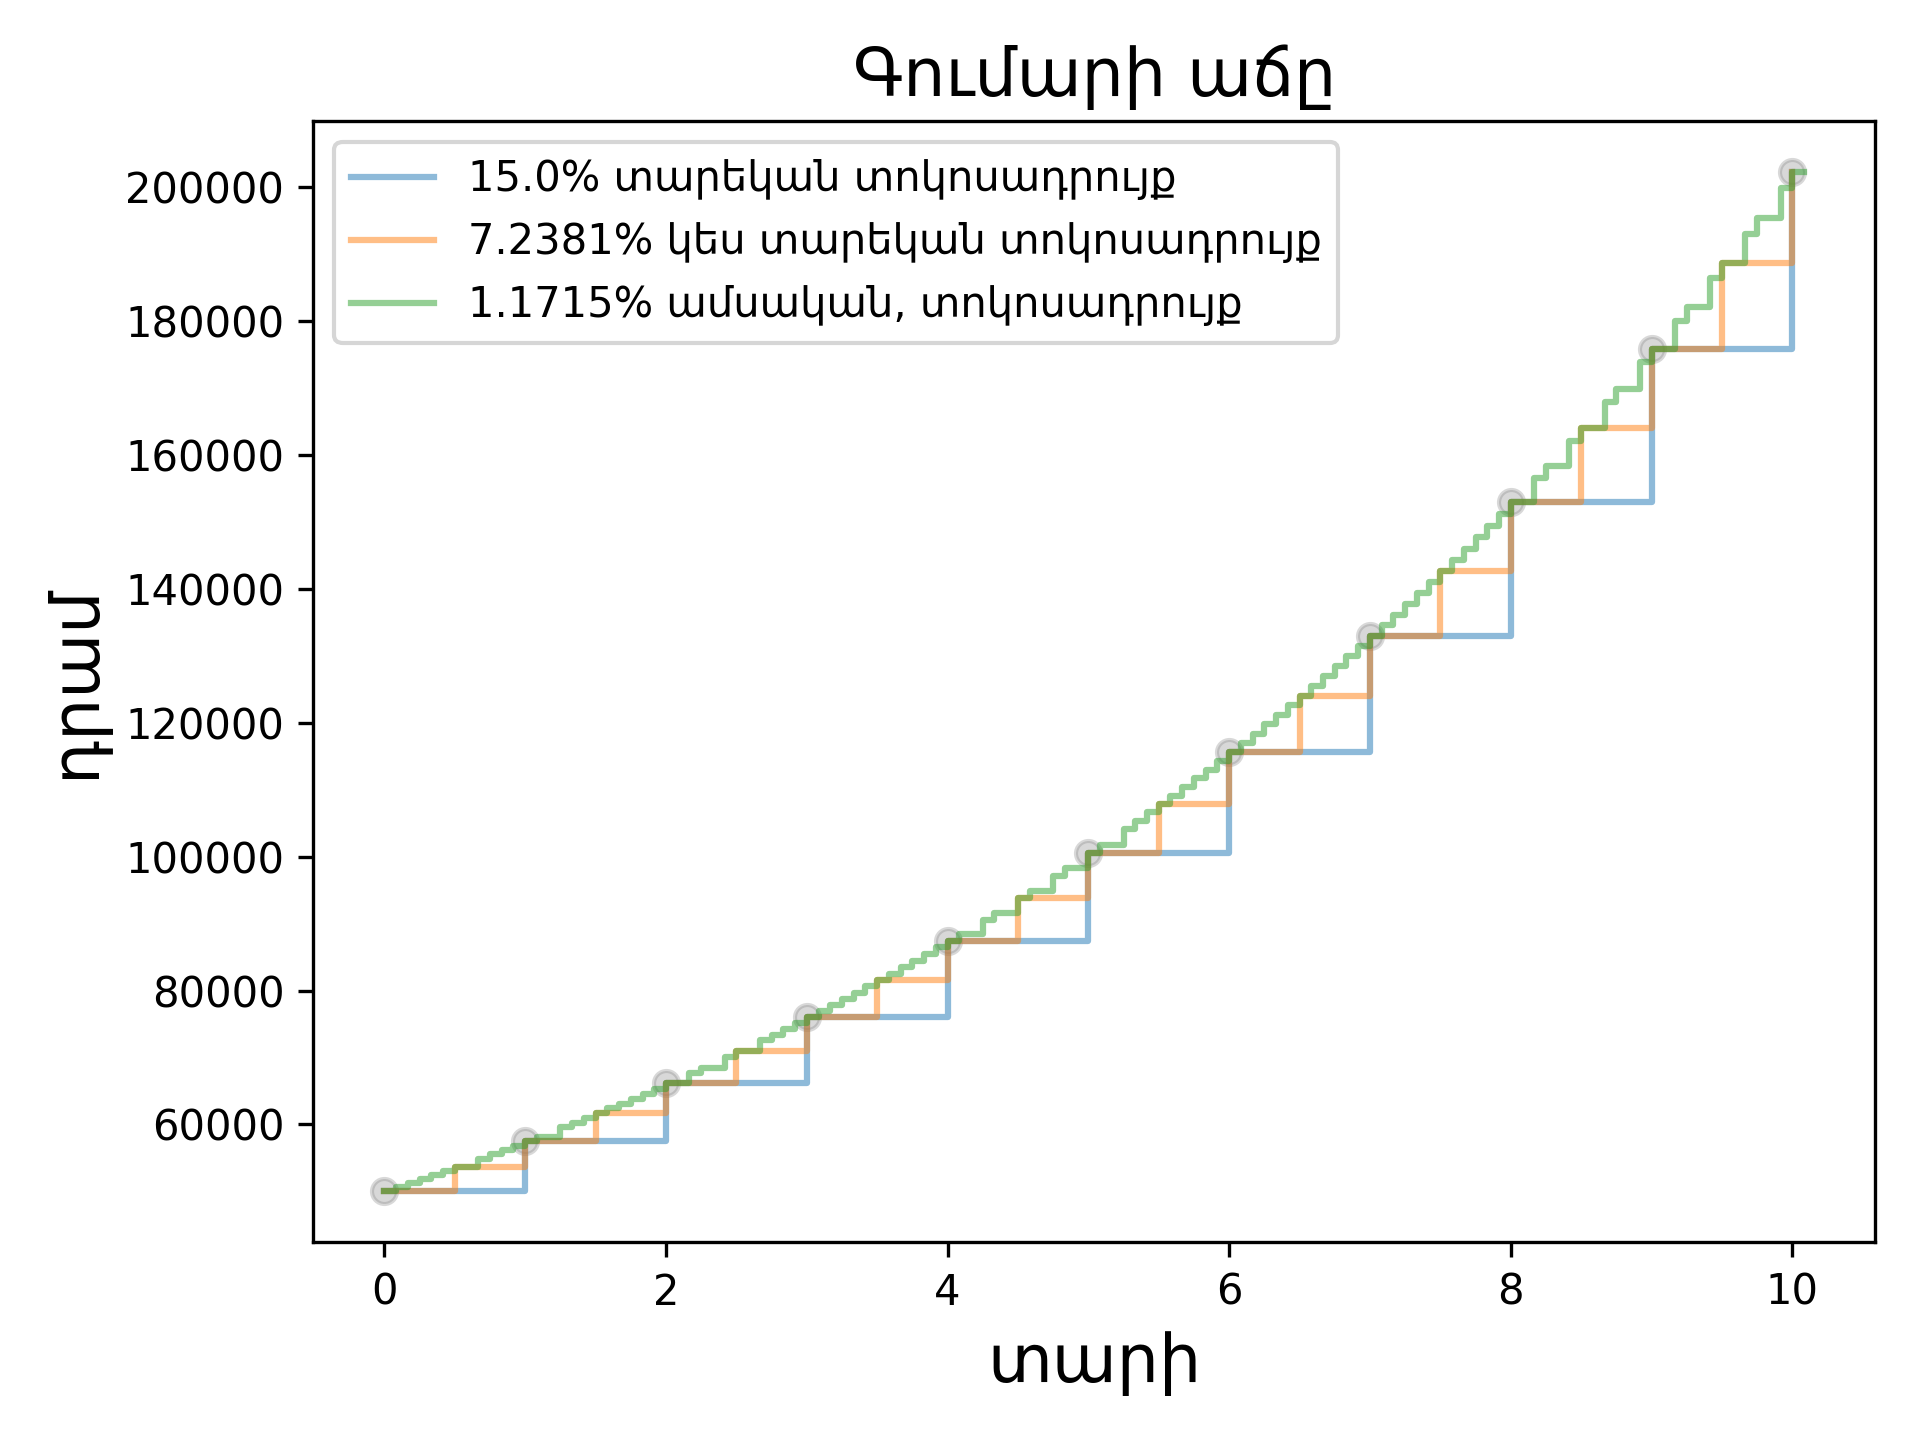
\includegraphics[width=0.4\textwidth]{1_2_12_0x100.png}
	    		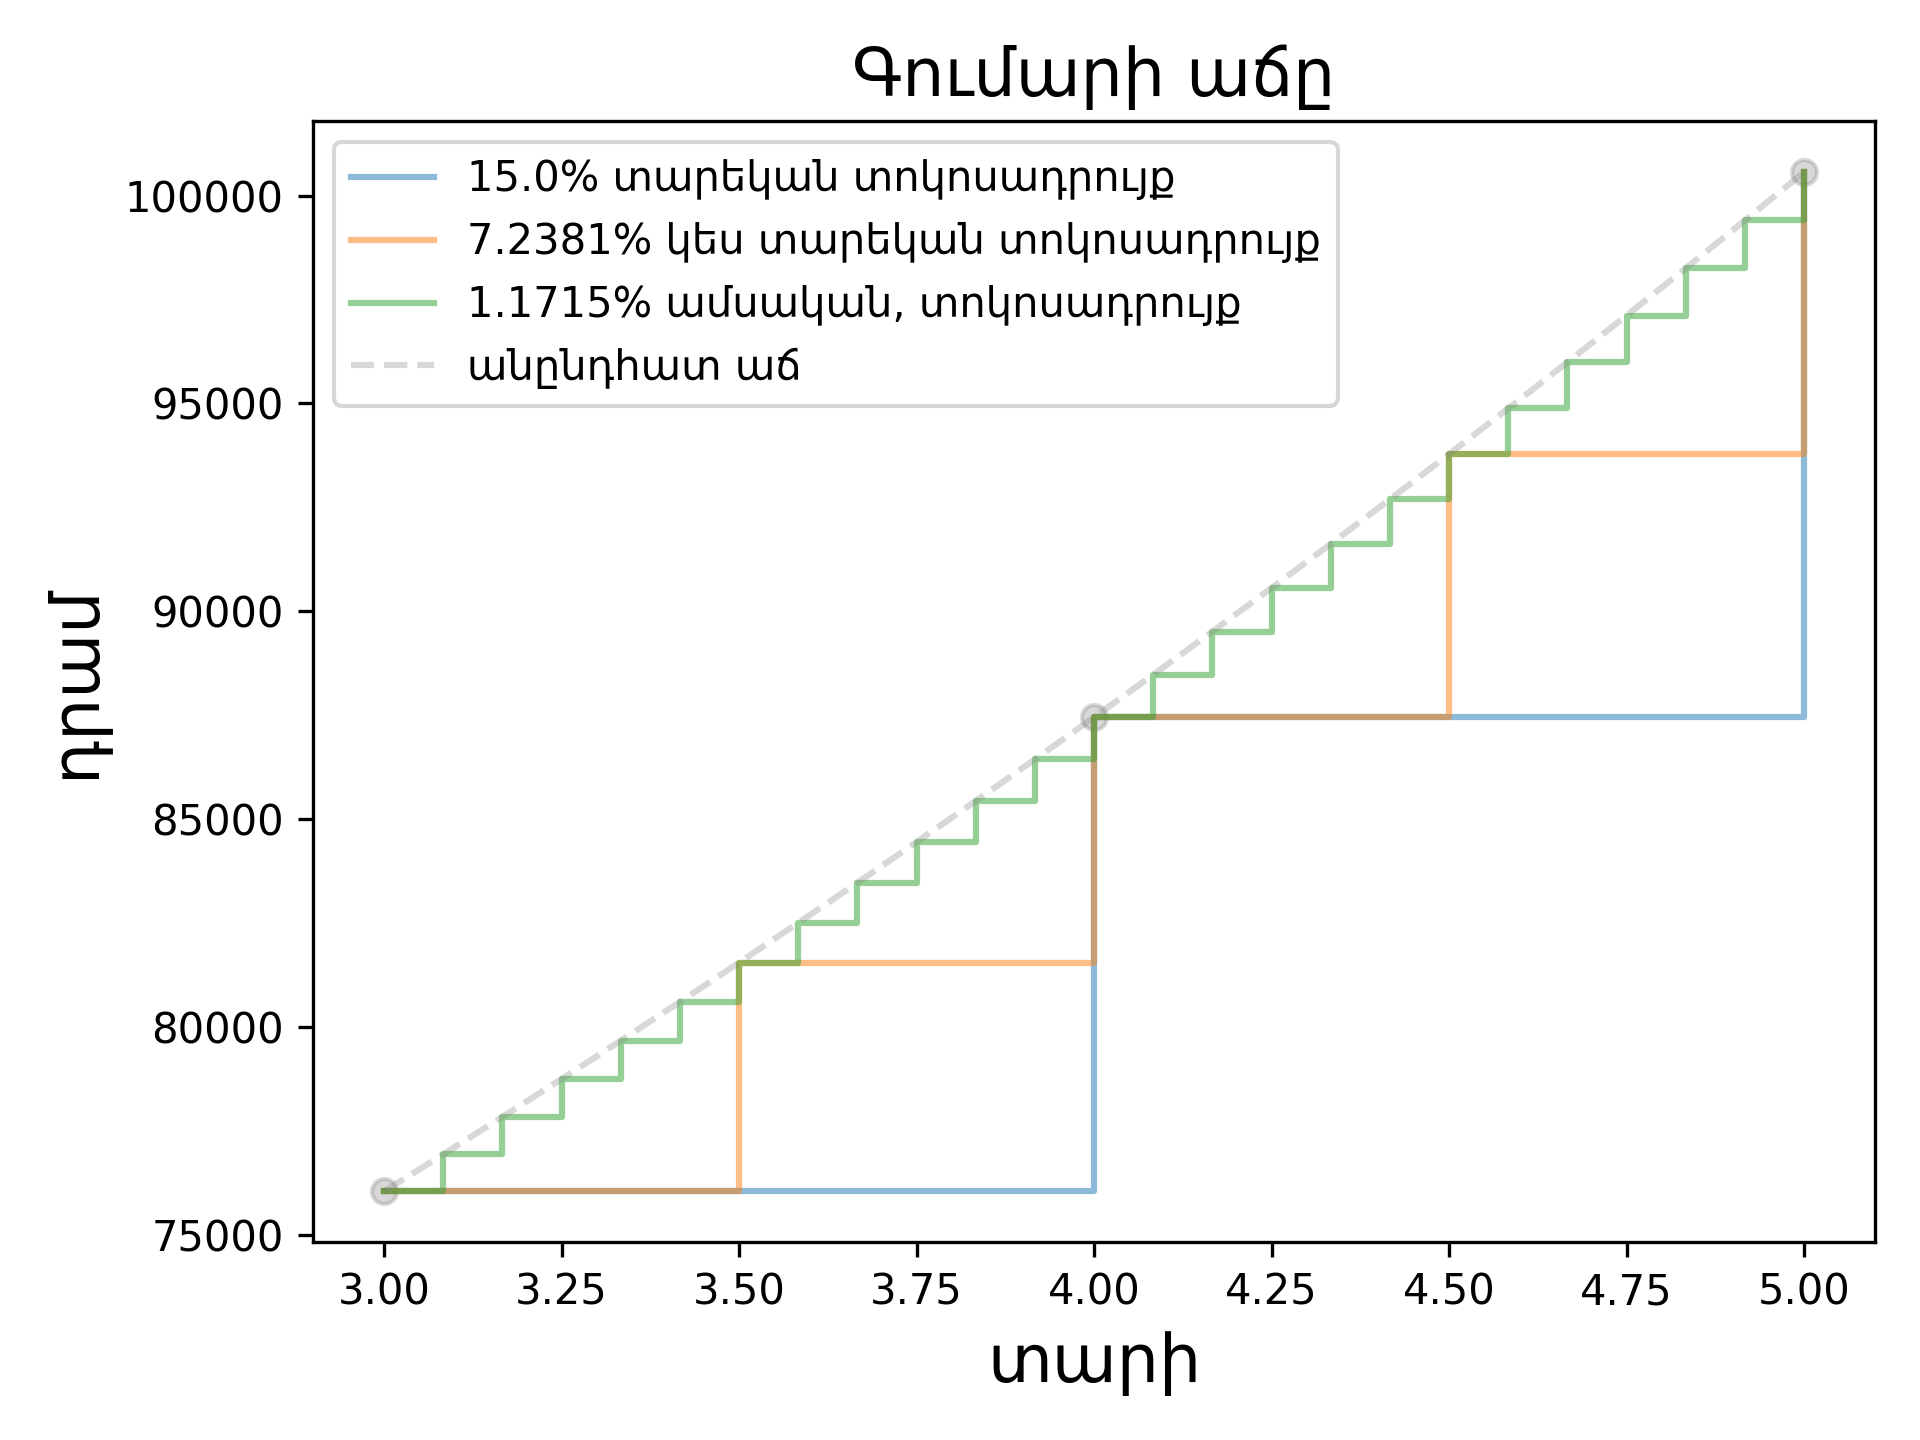
\includegraphics[width=0.4\textwidth]{1_2_12_30x50_c.png}
    		}
	    }
    \end{frame}
    \begin{frame}
        \frametitle{«Աքիլլեսն ու կրիան»}
        \framesubtitle{Մեկ, երկու, երեք, ․․․ \textcolor{red}{անվերջ}}
        \begin{columns}
        \only<1>{
            \column{0.5\textwidth}
            \noindent Որպես փուլ կհամարենք, երբ Աքիլլեսը հասնում է կրիայի սկզբնական դիրքին։
            \column{0.5\textwidth}
            \centering
            
\includegraphics[width=0.9\textwidth]{zeno_achilles_paradox_0.png}
        }
        \only<2>{
            \column{0.5\textwidth}
            \noindent $1$-ին փուլ
            \column{0.5\textwidth}
            \centering
            
\includegraphics[width=0.9\textwidth]{zeno_achilles_paradox_1.png}
        }
        \only<3>{
            \column{0.5\textwidth}
            \noindent $2$-րդ փուլ
            \column{0.5\textwidth}
            \centering
            
\includegraphics[width=0.9\textwidth]{zeno_achilles_paradox_2.png}
        }
        \only<4-5>{
            \column{0.5\textwidth}
            \only<5>{\noindent այսպես շարունակ, փուլերը անդաթար շարունակվում են}
            \only<4>{\noindent $3$-րդ փուլ}
            \column{0.5\textwidth}
            \centering
            
\includegraphics[width=0.9\textwidth]{zeno_achilles_paradox_3.png}
        }
        \only<6>{
            \column{0.5\textwidth}
            \noindent բոլոր փուլերը տեղի ունեցած են
            \column{0.5\textwidth}
            \centering
            
\includegraphics[width=0.9\textwidth]{zeno_achilles_paradox_i.png}
        }
        \end{columns}
    \end{frame}
    \begin{frame}
        \frametitle{Սահմանային անցում}
        ի՞նչպես կատարել սահմանային անցում
        \framesubtitle{Մեկ, երկու, երեք, ․․․ \textcolor{red}{անվերջ}}
        \begin{columns}
            \column{0.5\textwidth}
            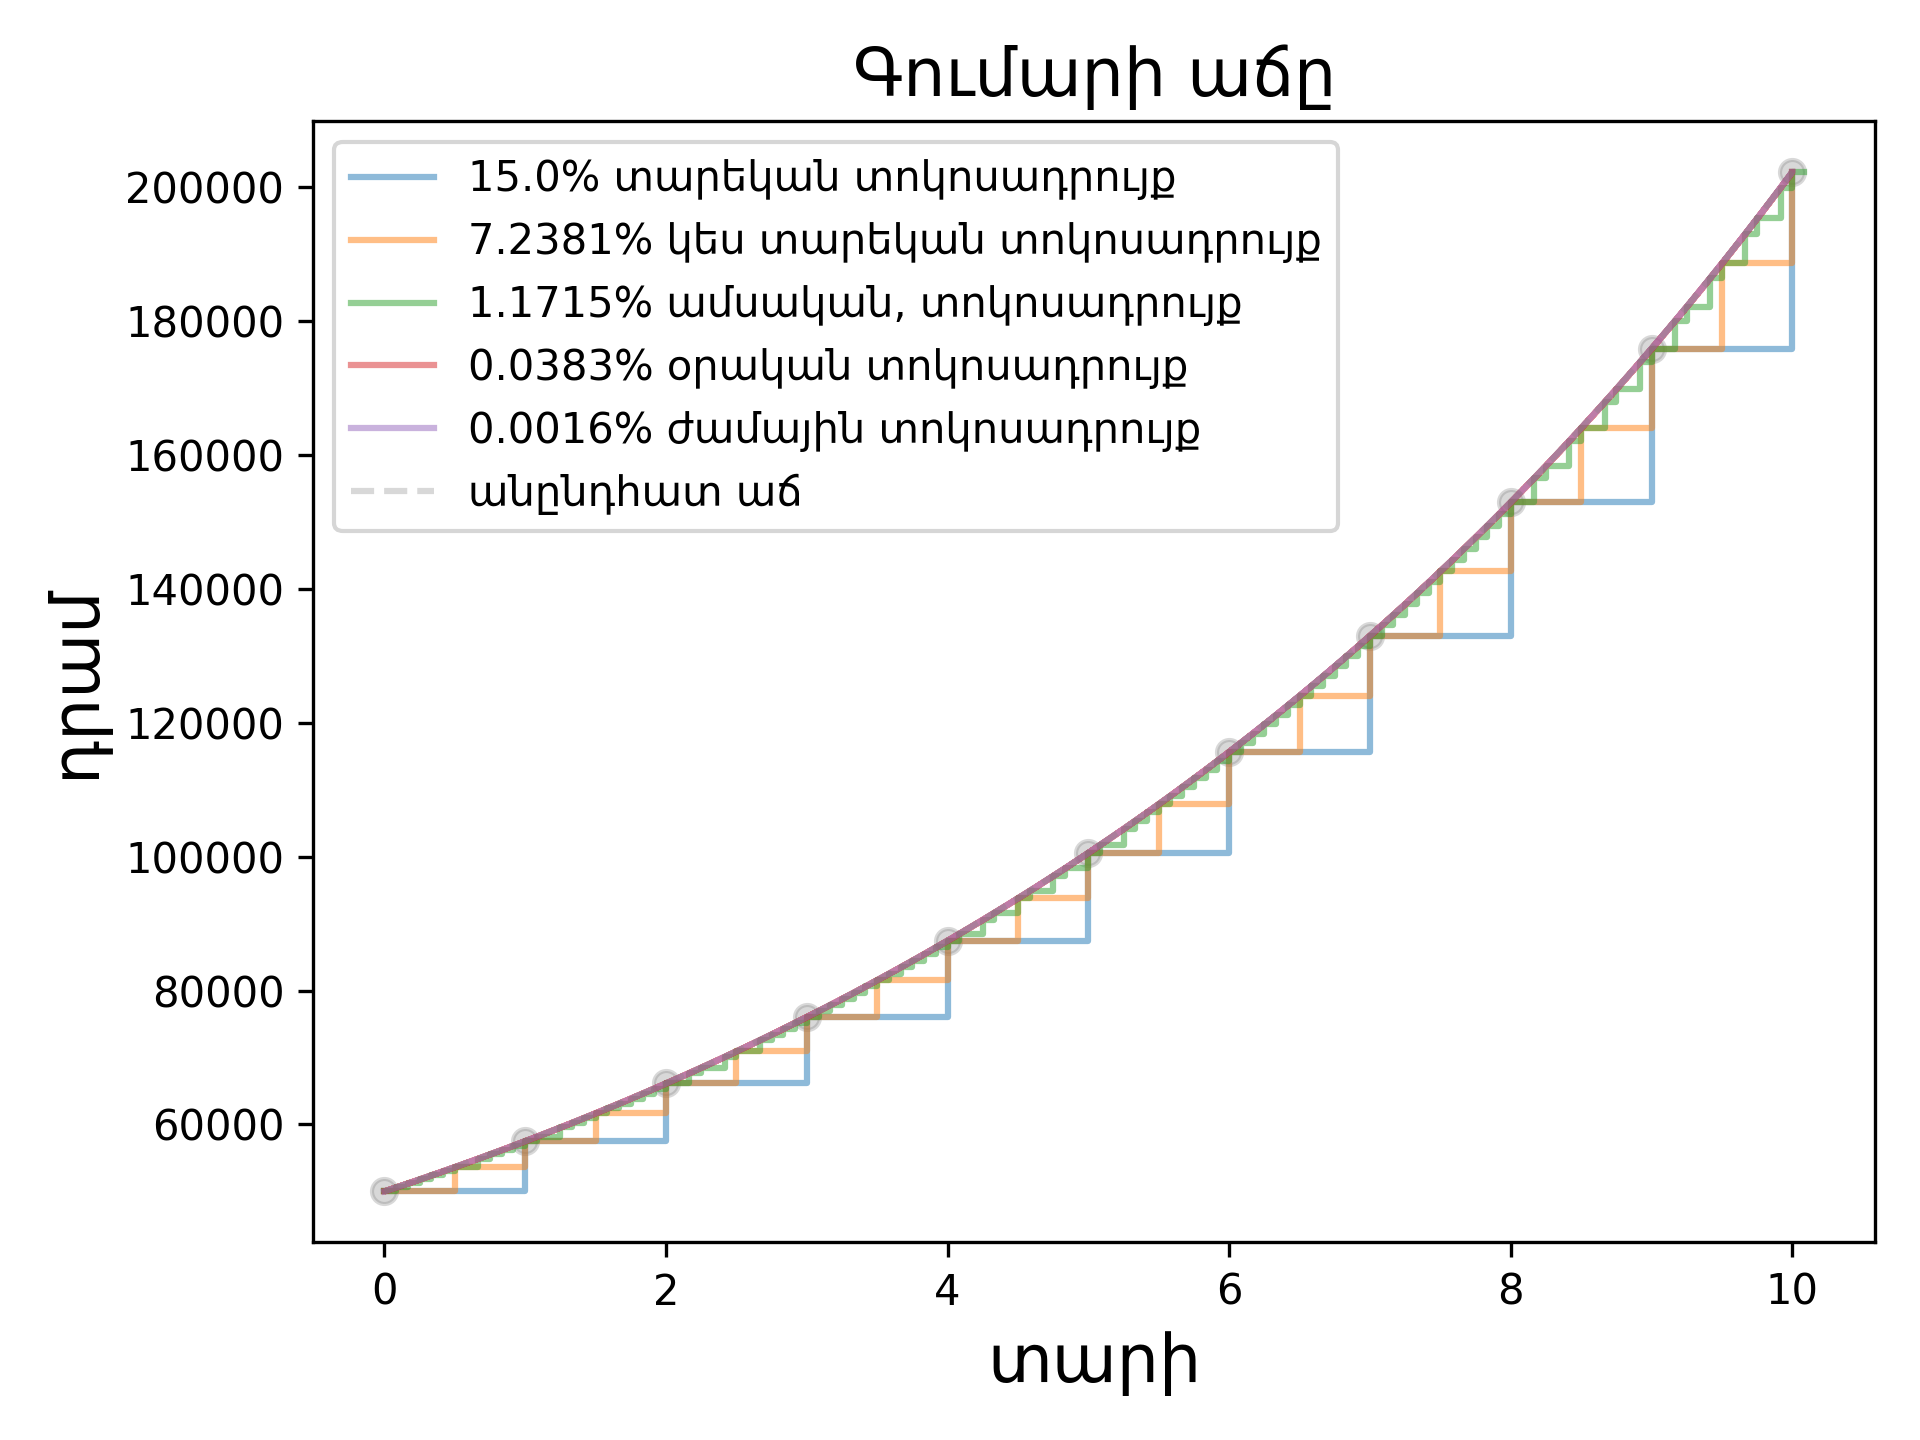
\includegraphics[width = 0.9\textwidth]{1_2_12_365_8766_0x100_c.png}
            \column{0.5\textwidth}
            
\includegraphics[width = 0.9\textwidth]{zeno_achilles_paradox_i.png}
        \end{columns}
    \end{frame}
     %%%%%%%   հաջորդականություն   %%%%%%%
    \subsection{հաջորդականություն}
    \begin{frame}
        \frametitle{Հաջորդականություն}
        \framesubtitle{Բնական թվեր}
        $\mathbb{N} = \{1, 2, 3, ...\}$
        \only<2->{\begin{block}{Հատկություններ}
            \begin{itemize}
                \only<2->{
                    \item Բնական թվերը կարգավորված են.\\
                    կամայական երկու բնական թվեր կարող ենք համեմատել
                    \only<3->{\\ օրինակ՝ $57 \le 234$}
                }
                \only<4->{
                    \item Բնական թվերը անվերջ շատ են.\\
                    կամայական բնական թվին կա հաջորդող բնական թիվ
                    \only<5->{\\ օրինակ՝ $1991$-ին հաջորդում է $1992$}
                }
                \only<6->{
                    \item Բնական թվերից կազմված \textcolor<8-9>{red}{կամայական}  բազմություն, այսինքն՝ \textcolor<9>{red}{բնական թվերի ենթաբազմությունը} \textcolor<10>{red}{ունի} \textcolor<11>{red}{ամենափոքր թիվը}.
                    \only<7->{\\ $\textcolor<8-9>{red}{\forall} \textcolor<9>{red}{A \subset \mathbb{N}} \; \textcolor<10>{red}{\exists n \in A} \; \textcolor<11>{red}{\forall m \in A \; n \le m}$}
                }
            \end{itemize}
        \end{block}}
    \end{frame}
	\begin{frame}
        \frametitle{Հաջորդականություն}
        \only<1-2, 6-7>{\begin{block}{Սահամնում}
            \alert<1>{Հաջորդականություն} ենք անվանում $a: \mathbb{N} \to \mathbb{R}$ ֆունկցիան։ $a(n)$-ի փոխարեն գրելու ենք $a_n$, իսկ հաջորդականությունը եբեմն $(a_n)$
        \end{block}}
        \only<2-5>{
            \begin{exampleblock}{Օրինակ}
                Հայկի ստացած գումարը տարվա $\pi$-րդ պահին, եթե տարեկան $n$ անգամ գումարը աճեր․
                \[a_n = 50000 \left(\sqrt[n]{1+\frac{15}{100}}\right)^{[n\pi]},\] որտեղ $[x]$-ը $x$ թվի ամբողջ մասն է։
            \end{exampleblock}
            \only<3>{\[a_{10} =\]}
            \only<4>{\[a_{10} = 50000 \left(\sqrt[10]{1+\frac{15}{100}}\right)^{31}\]}
            \only<5>{\[a_{10} = 50000 \left(1+\frac{15}{100}\right)^{3.1}\]}
            }
        \only<6>{\centering{
            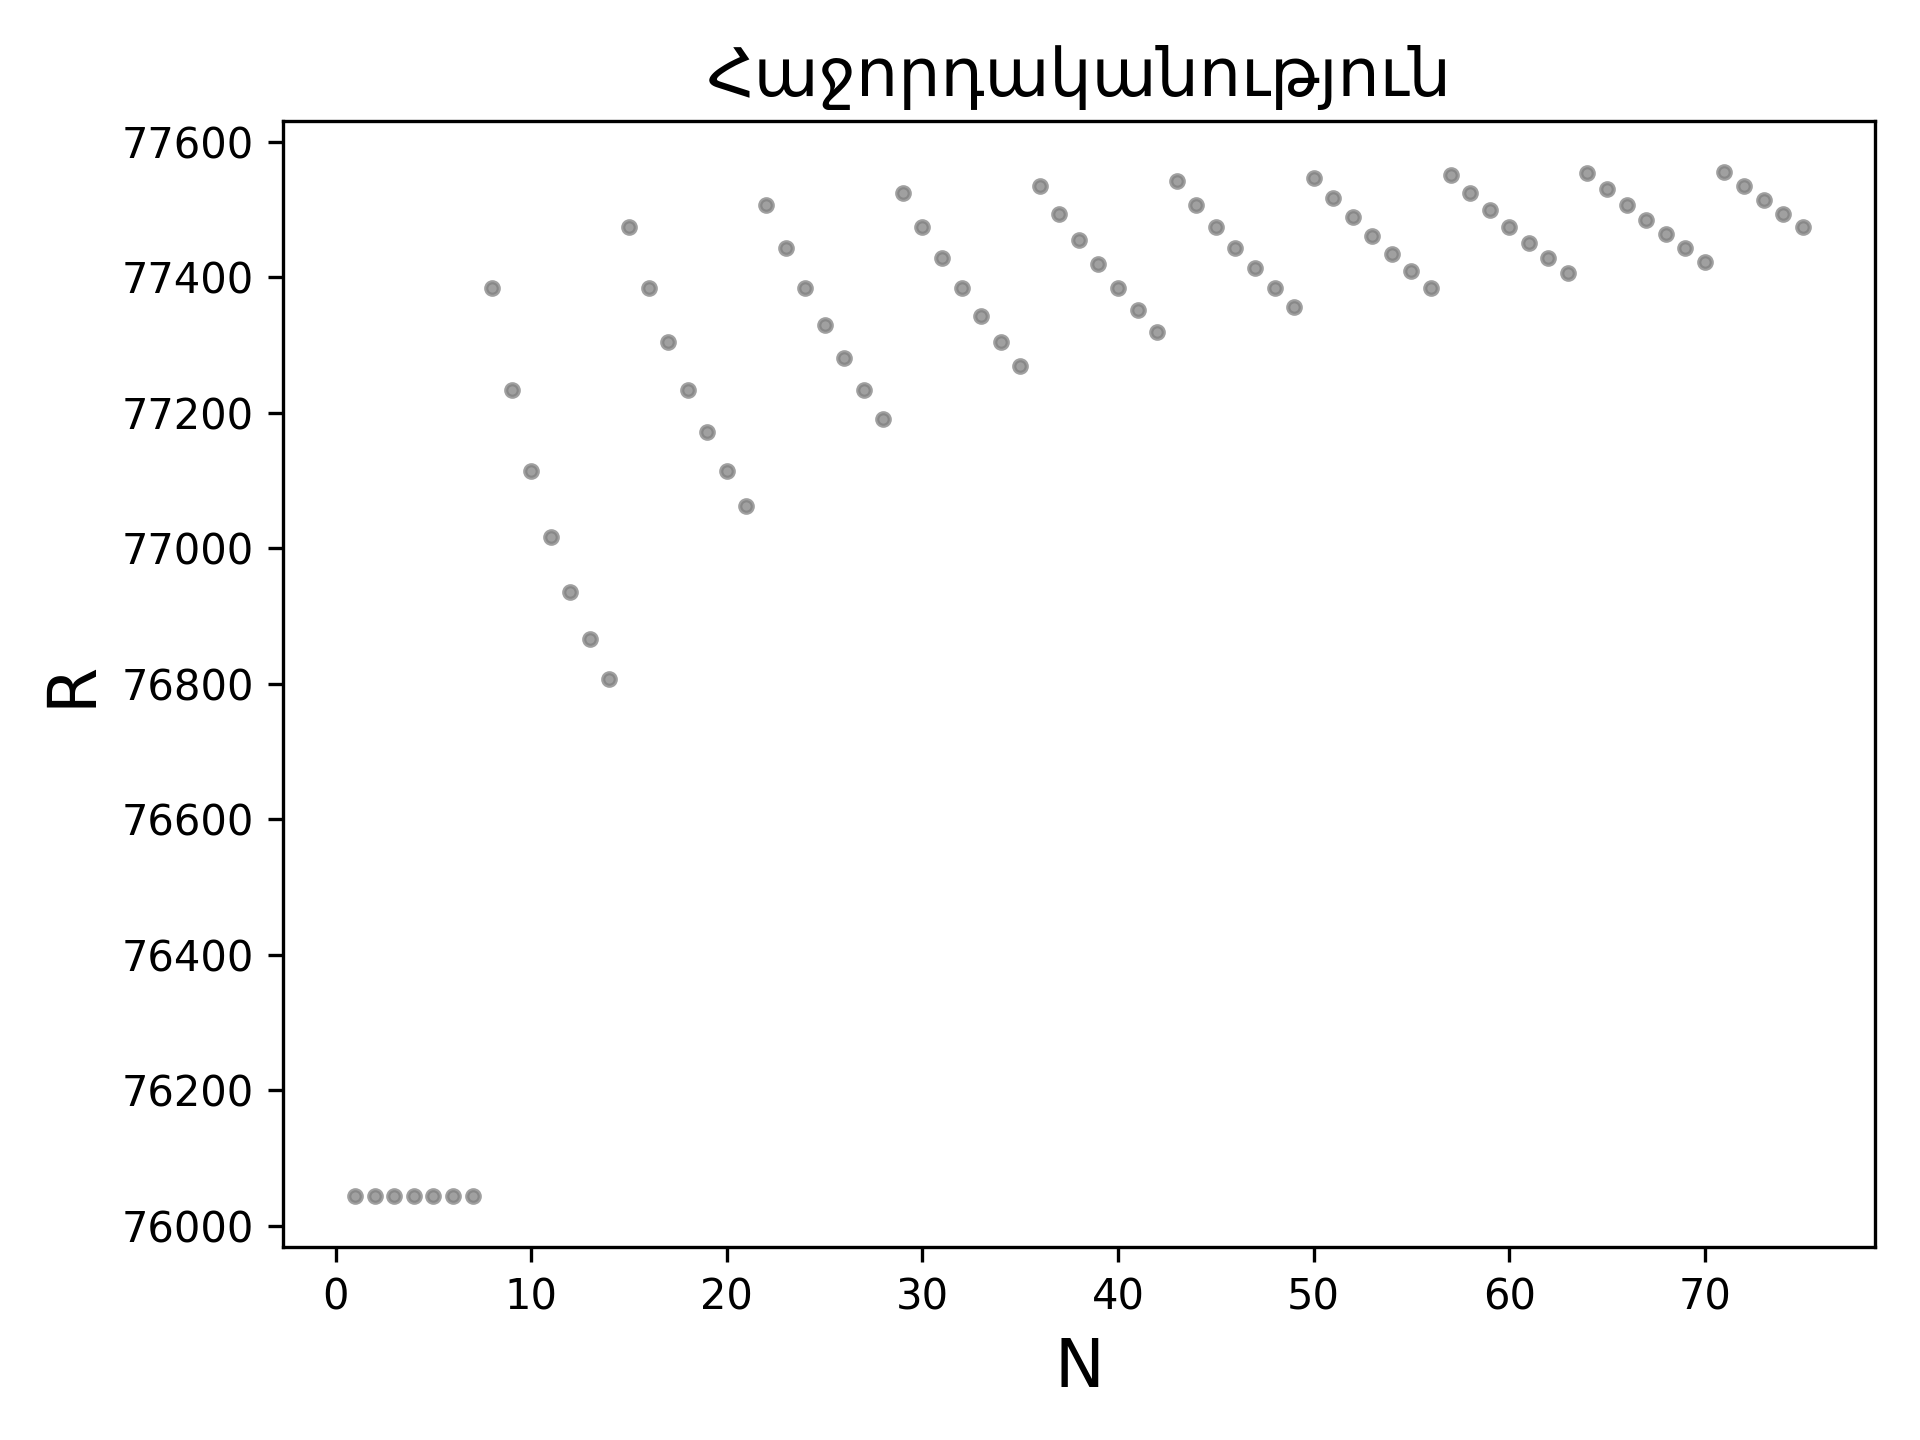
\includegraphics[width=0.4\textwidth]{sequence_c.png}
        }}
        \only<7->{
            \begin{exampleblock}{Օրինակ}
                $\pi$ թիվը մինչև $n$-րդ նիշը
                \[a_n = \frac{[10^{n-1} \pi]}{10^{n-1}},\] որտեղ $[x]$-ը $x$ թվի ամբողջ մասն է։
            \end{exampleblock}
            \only<8>{\[a_{1} = 3\]}
        	\only<9>{\[a_{2} = 3.1\]}
        	\only<10>{\[a_{3} = 3.14\]}
        	\only<11>{\[a_{4} = 3.141\]}
        	\only<12>{\[a_{5} = 3.1415\]}
            \only<13->{
        		Նկատենք, որ՝
        		\[\only<14->{0 \le } a_{\only<13-15>{8} \only<16>{m}} - a_{\only<13-15>{5} \only<16>{n}} \only<15>{ \le 10^{-3} = 0.001} \only<16->{ \le 10^{-n + 2} = 0.\underbrace{0 \dots01}_{n-2 \text{ հատ}},}\] \only<16>{որտեղ $m \ge n$:}
        	}
    	}
    \end{frame}
    \begin{frame}
        \frametitle{Ֆունդամենտալ հաջորդականություն}
   		\begin{block}{Սահամնում}
   			Կասենք, որ $(a_n)$ հաջորդականությունը \alert<1>{ֆունդամենտալ} է, եթե՝ \textcolor<3>{red}{ինչքան ասես փոքր է} լինում \textcolor<4>{red}{սկսած ինչ֊որ պահից} հաջորդականության \textcolor<5>{red}{կամայական երկու անդամենրի տարբերության բացարձակ արժեքը}.
   			\only<2->{\[\textcolor<3>{red}{\forall \varepsilon > 0} \quad \textcolor<4>{red}{\exists N_{\varepsilon} \in \mathbb{N}}: \quad \textcolor<5>{red}{\forall n, m} \textcolor<4>{red}{> N_{\varepsilon}} \quad \textcolor<5>{red}{|a_n - a_m|} \textcolor<3>{red}{< \varepsilon}:\]}
   		\end{block}
   		\only<6>{
            \begin{exampleblock}{Օրինակ}
                Հաջորդականությունը, որտեղ $n$-րդ անդամը $\frac{[10^{n-1} \pi]}{10^{n-1}}$ է՝ ֆունդամենտալ է։
            \end{exampleblock}
        }
    \end{frame}
    \begin{frame}
        \frametitle{Ֆունդամենտալ հաջորդականություն}
        \framesubtitle{Հաջորդականություն սահմանափակությունը}
        \only<1-7>{
            \begin{block}{Սահամնում}
                Կասենք, որ $(a_n)$ հաջորդականությունը \alert<1-2>{սահմանափակ} է, եթե՝ $a$-ի արժեքների տիրույթը՝ $a(\mathbb{N})=\{a(n): n \in \mathbb{N}\}$, \alert<2>{սահմանափակ բազմություն} է:
            \end{block}
        }
        \only<3-8>{
            \begin{block}{Սահամնում}
                Կասենք, որ $A$ \alert<3>{բազմությունը սահմանափակ} է, եթե \alert<4>{կա այնպիսի թիվ}, որ \alert<5>{$A$ բազմությանը պատկանող կամայական թվի} բցարձակ արժեքից \alert<4>{մեծ կամ հավասար է}.
                \only<4->{\[\alert<4>{\exists M \in \mathbb{R}} : \alert<5>{\forall a \in A} \quad |a| \alert<4>{\leq M}:\]}
            \end{block}
            \only<6->{
                \begin{exampleblock}
                    \only<6->{$\left(\frac{1}{n}\right)$ հաջորդականությունը սահմանափակ է։\\}
                    \only<7->{$\left(\frac{n^3}{2-n^2}\right)$ հաջորդականությունը անսահմանափակ է։\\}
                \end{exampleblock}
                \only<8>{$\frac{n^3}{2-n^2} = \frac{n}{\frac{2}{n^2}-1} < -\frac{n}{10}$ երբ $n > 1$}
            }
        }
        \only<9->{
            \only<1-15, 21->{\begin{block}{Պնդում}
                Ֆունդամենտալ հաջորդականությունը սահմանափակ է։
            \end{block}}
        }
        \only<10->{
            \begin{alertblock}{Ապացույց}
                Դիցուք՝ $(a_n)$ հաջորդականությունը ֆունդամենտալ է։
                \only<11-12>{Ունենք որ՝ ինչքան ասես փոքր է սկսած ինչ-որ պահից կամայական երկու անդամենրի տարբերության բացարձակ արժեքը։}
                \only<12-15>{\only<8->{{Ունենք որ՝}\[\forall \varepsilon > 0 \; \exists N_{\varepsilon} \in \mathbb{N} \; \forall n, m > N_{\varepsilon} \; |a_n - a_m| < \varepsilon\]}}
                \only<13-15>{Մասնավոր դեպքում, $\varepsilon = 3$՝ ինչ-որ պահից սկսած հաջորդականության անդամների տարբերության տարբերությունը փոքր է $3$-ից․}
                \only<14>{\[\forall n, m > N_3 \; |a_n - a_m| < 3:\]}
                \only<15->{\only<16->{Ունենք որ՝} \[\forall n > N_3 \; |a_{N_3+1} - a_n| < 3\only<16->{:}\]}
                \only<21->{
                    \only<21->{Նշանակաենք $M$-ով $|a_1|, \; |a_2|,\; ..., \; |a_{N_3}|, \; |a_{N_3 + 1} + 3|, \; |a_{N_3 + 1} - 3|$ թվերից մեծագույնը}
                    \only<22->{Նկատենք, որ $(a_n)$ հաջորդականություն կամայական անդամի բացարձակ արժեքը փոքր կամ հավասար է $M$-ից․}
                    \only<23->{\[\forall n \in \mathbb{N} \; |a_n| \leq M:\]}
                }
            \end{alertblock}
        }
        \centering
            \only<16>{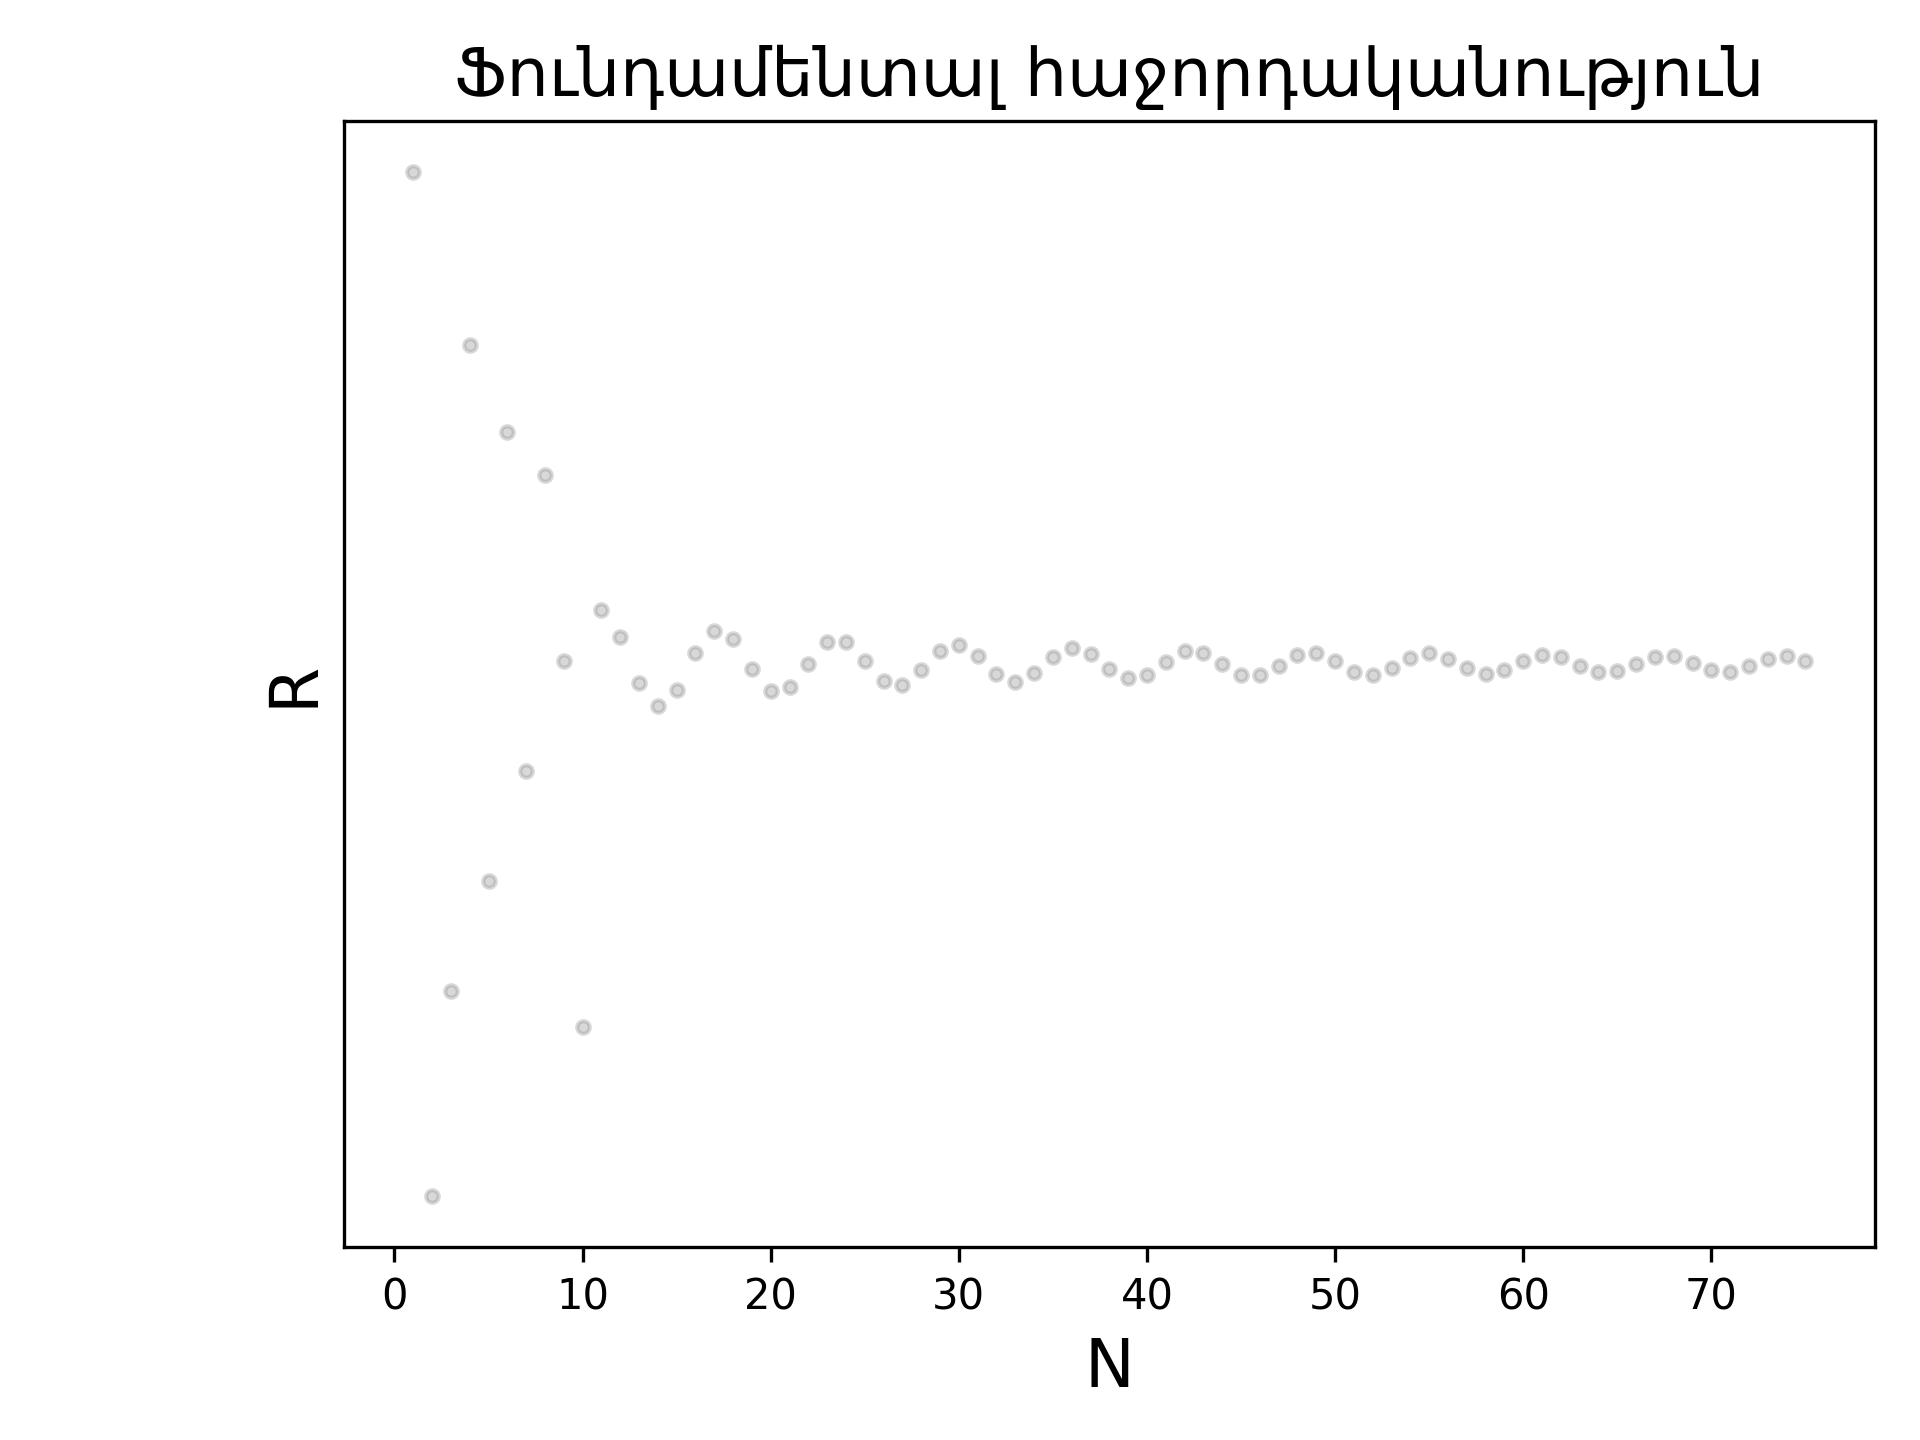
\includegraphics[width=0.4\textwidth]{sequence_boundness_fundamental_sequence_0.png}}
            \only<17>{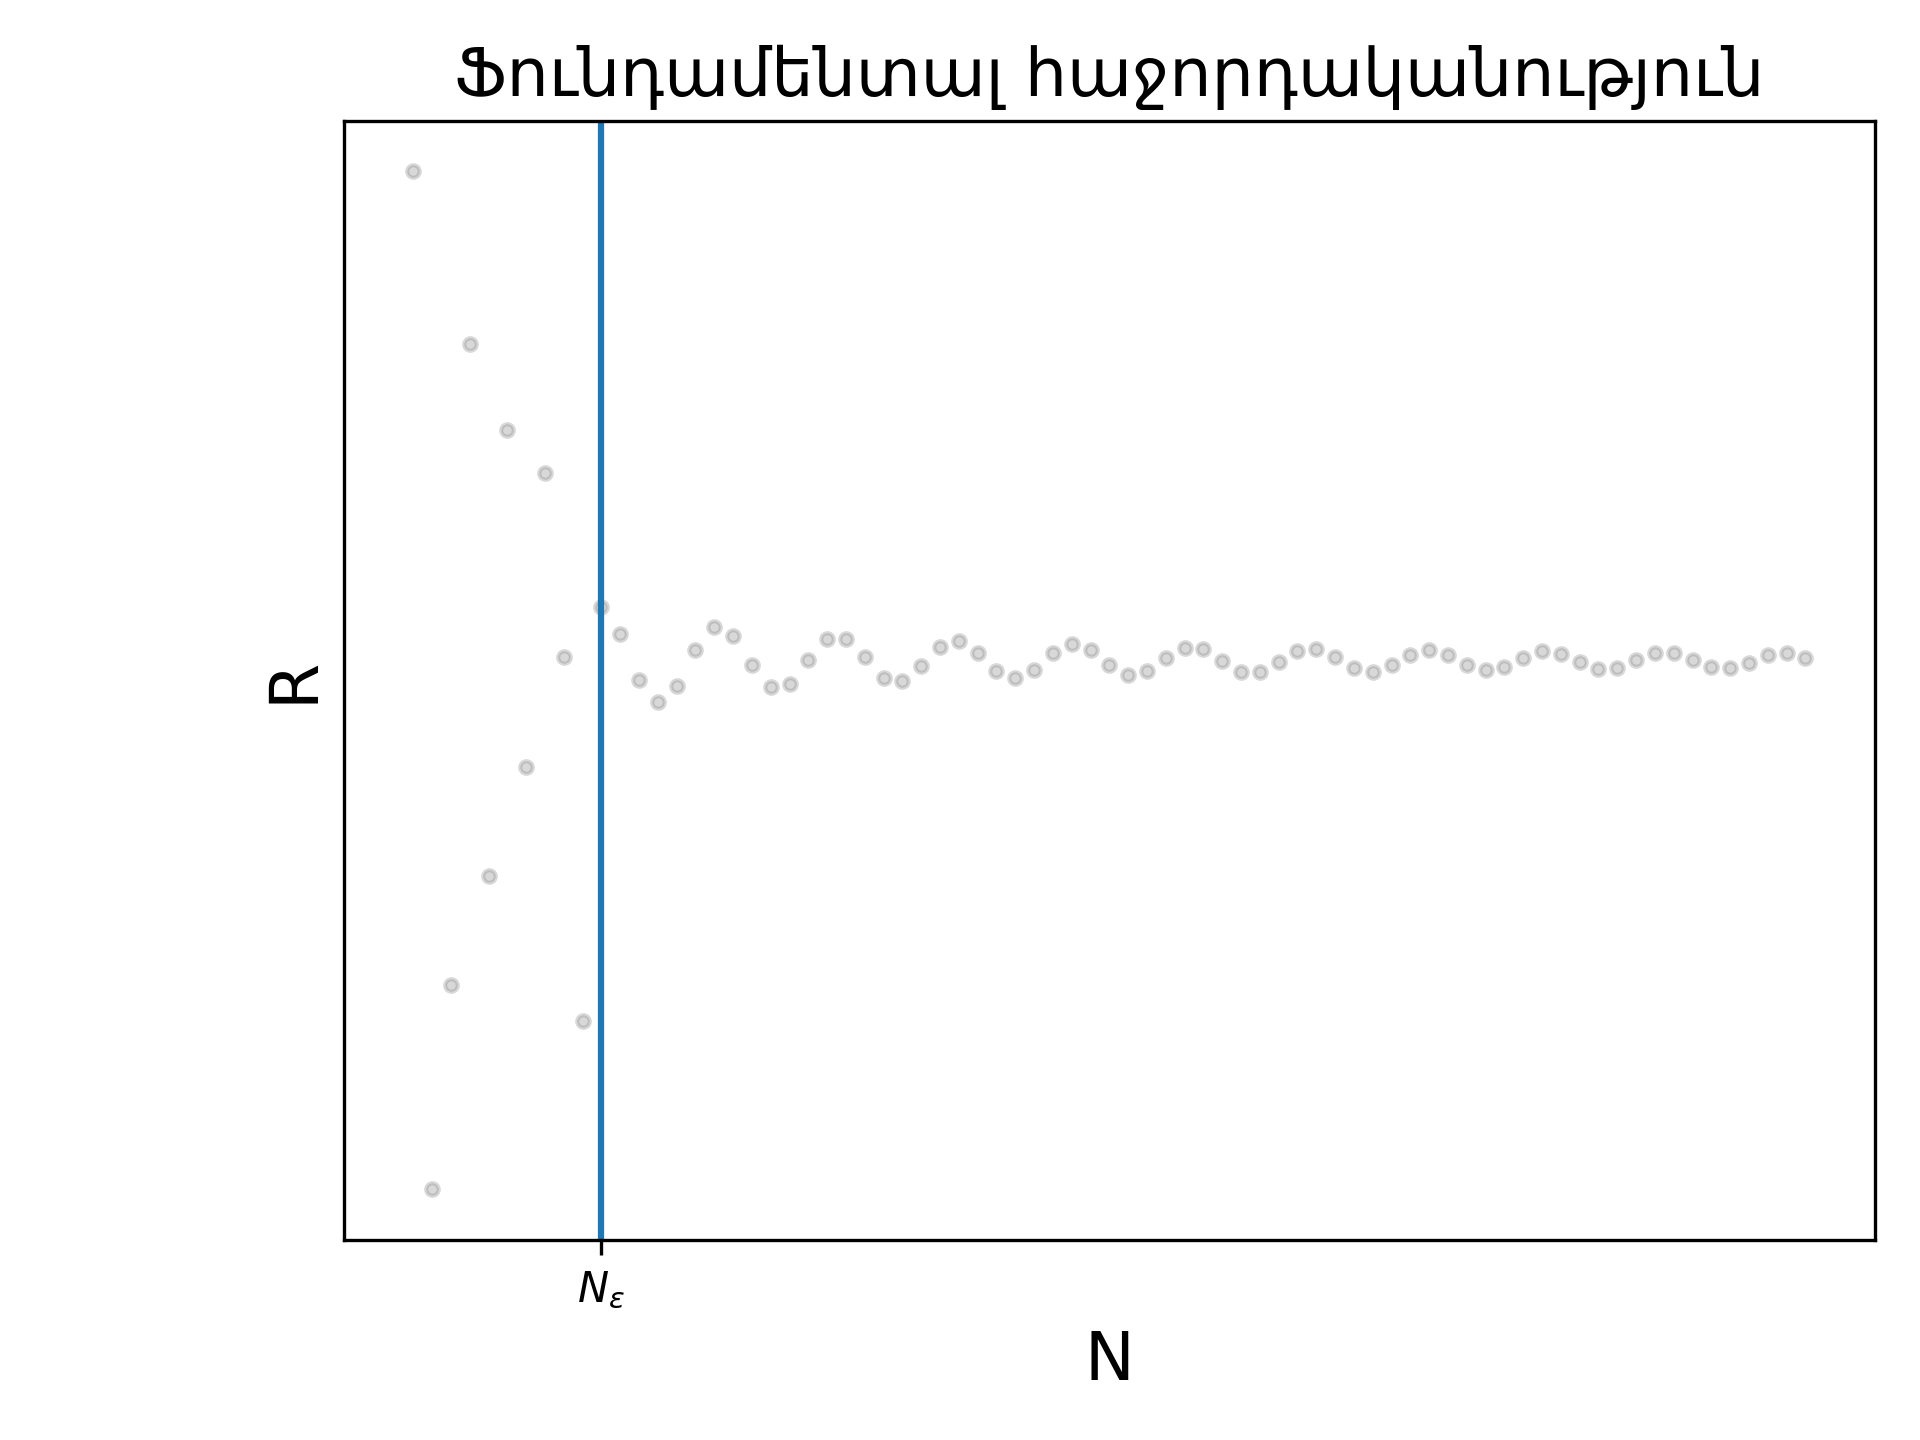
\includegraphics[width=0.4\textwidth]{sequence_boundness_fundamental_sequence_1.png}}
            \only<18>{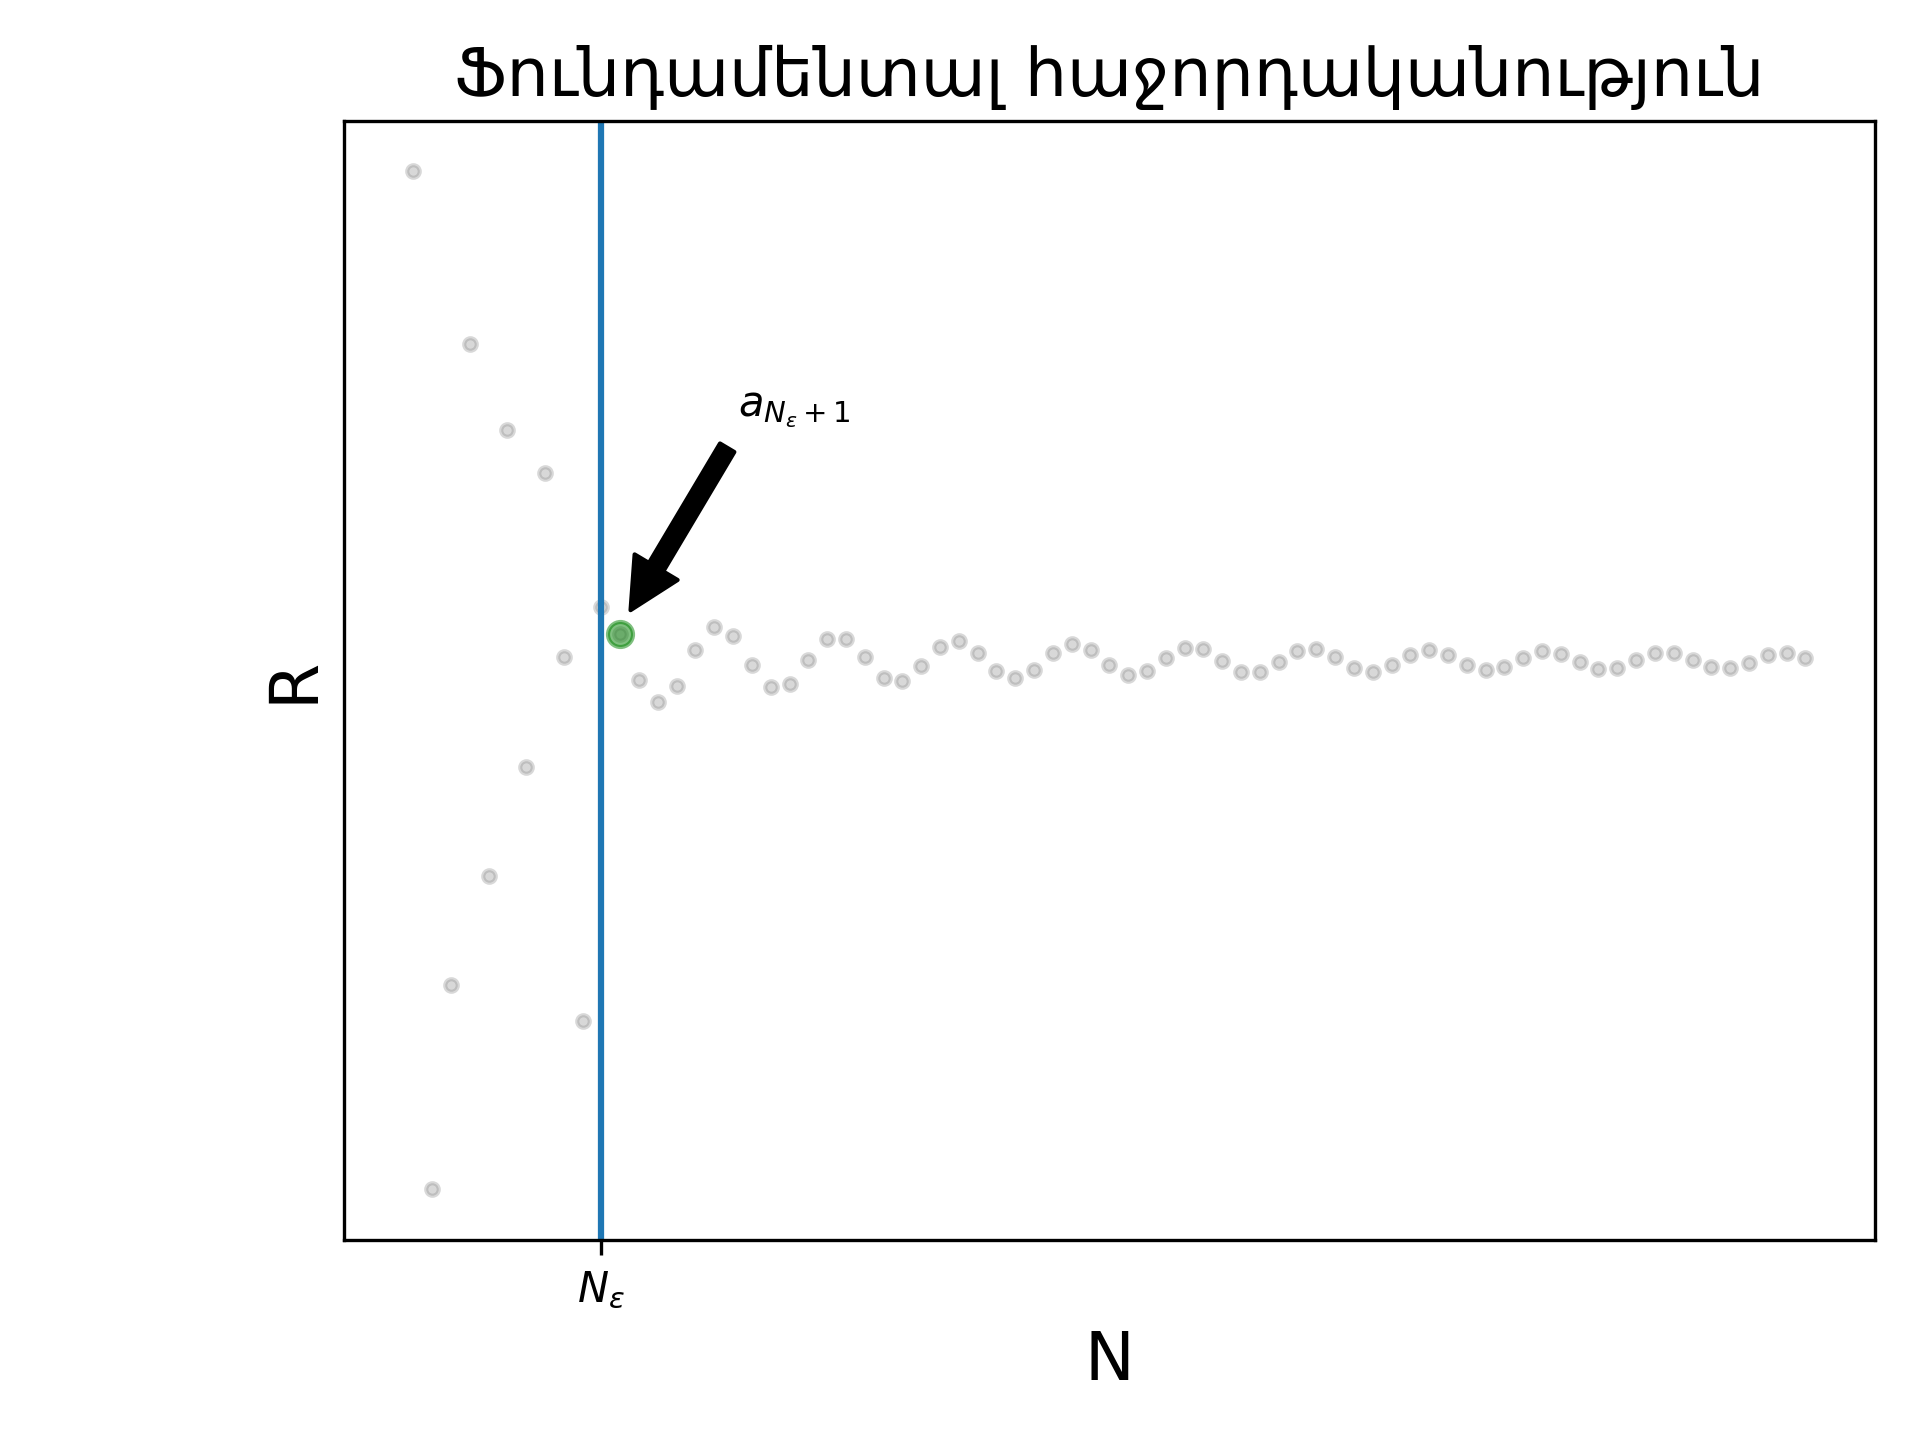
\includegraphics[width=0.4\textwidth]{sequence_boundness_fundamental_sequence_2.png}}
            \only<19>{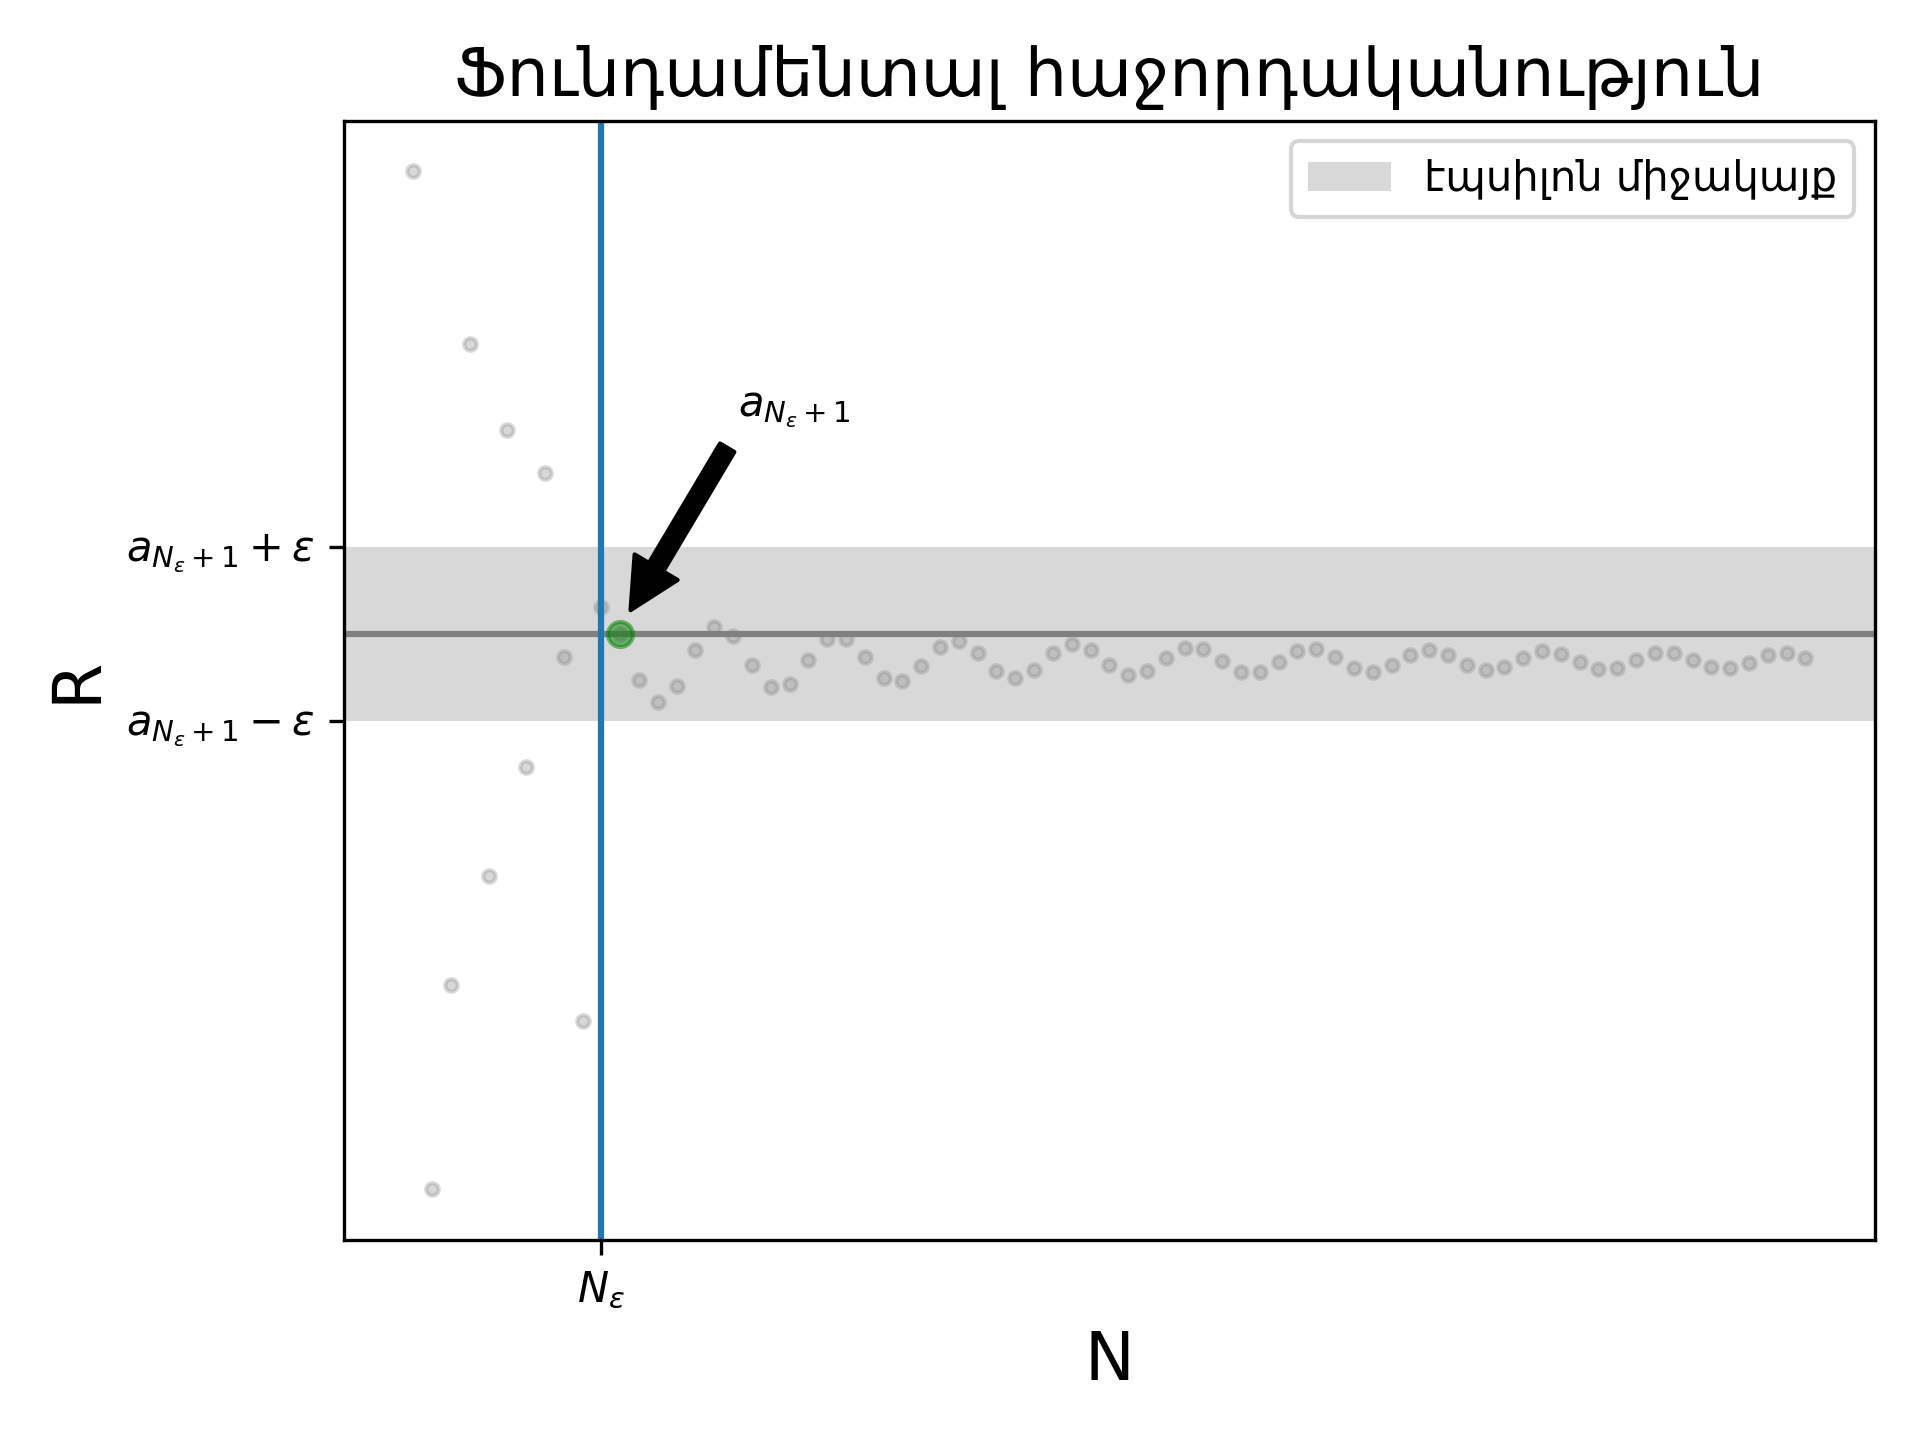
\includegraphics[width=0.4\textwidth]{sequence_boundness_fundamental_sequence_3.png}}
            \only<20>{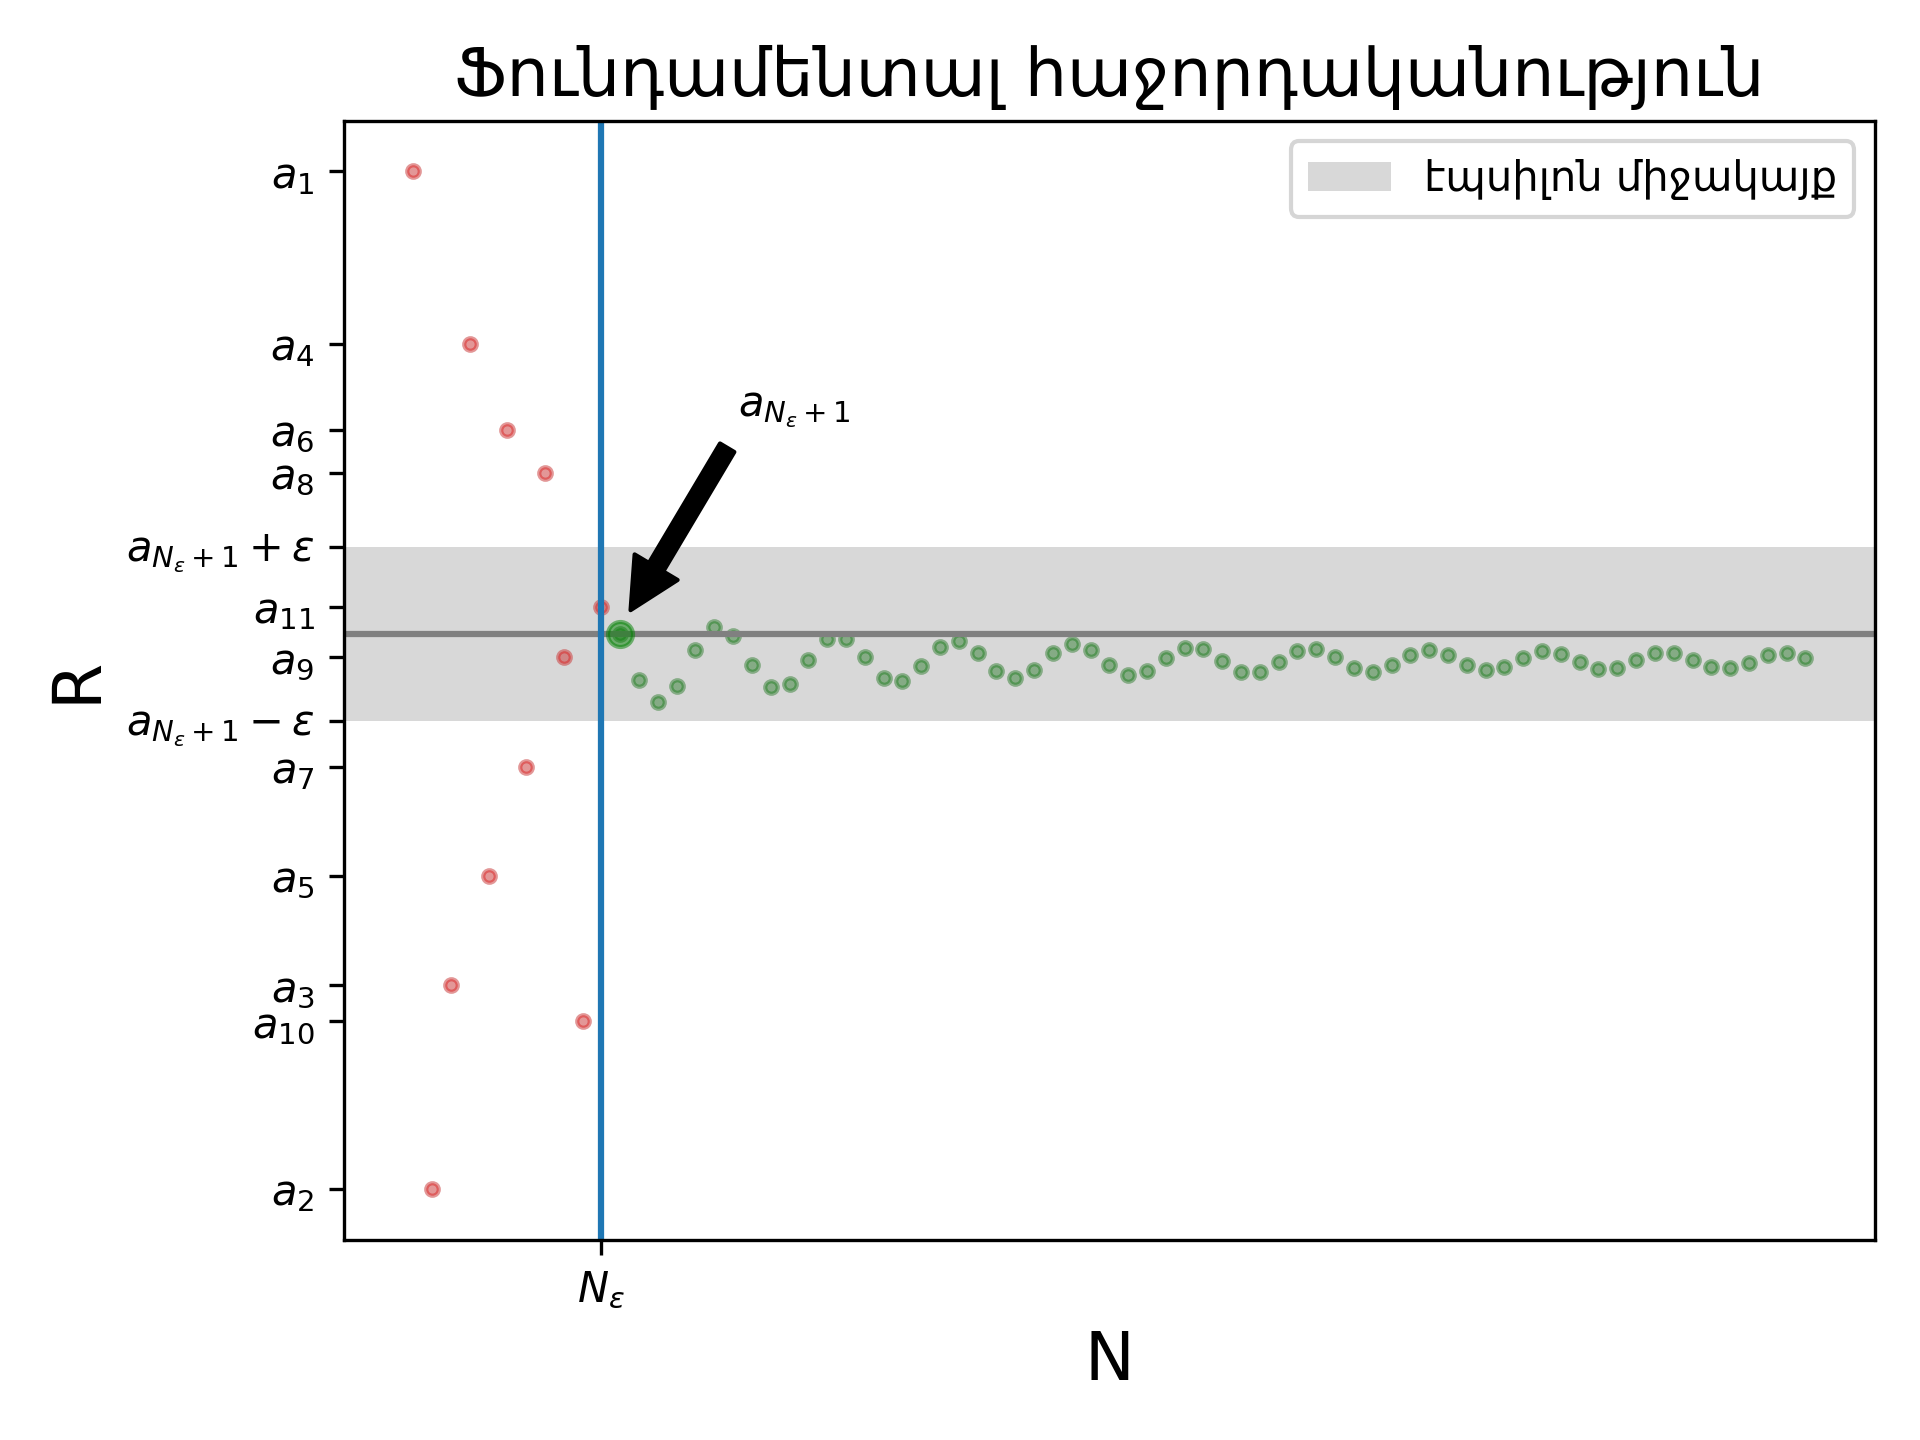
\includegraphics[width=0.4\textwidth]{sequence_boundness_fundamental_sequence_4.png}}
    \end{frame}
    \begin{frame}
        \frametitle{Ֆունդամենտալ հաջորդականություն}
        \framesubtitle{Հանրահաշվական գործողություններ}
        Դիցուք \textcolor<1-6>{seahorsegreen2}{$(a_n)$} և  \textcolor<1-6>{seahorseorange2}{$(b_n)$} հաջորդականությունները ֆունդամենտալ են։
        \only<2->{
            \begin{block}{Պնդում}
                Հետևյալ հաջորդականությունները ևս ֆունդամենտալ են․
                \only<3->{
                    \begin{itemize}
                        \only<3->{
                            \item \textcolor{seahorseblue2}{$(a_n + b_n)$}
                        }
                        \only<4->{
                            \item \textcolor{seahorsepink2}{$(a_n b_n)$}
                        }
                        \only<5->{
                            \item \textcolor{seahorsegray2}{$\left(a_n / b_n\right)$}, երբ $\exists \delta > 0: \; \exists N \in \mathbb{N} \; \forall n > N: \; |b_n| > \delta$
                        }
                    \end{itemize}
                }
            \end{block}
        }
        \only<1-6>{
            \centering{
                \only<1-2>{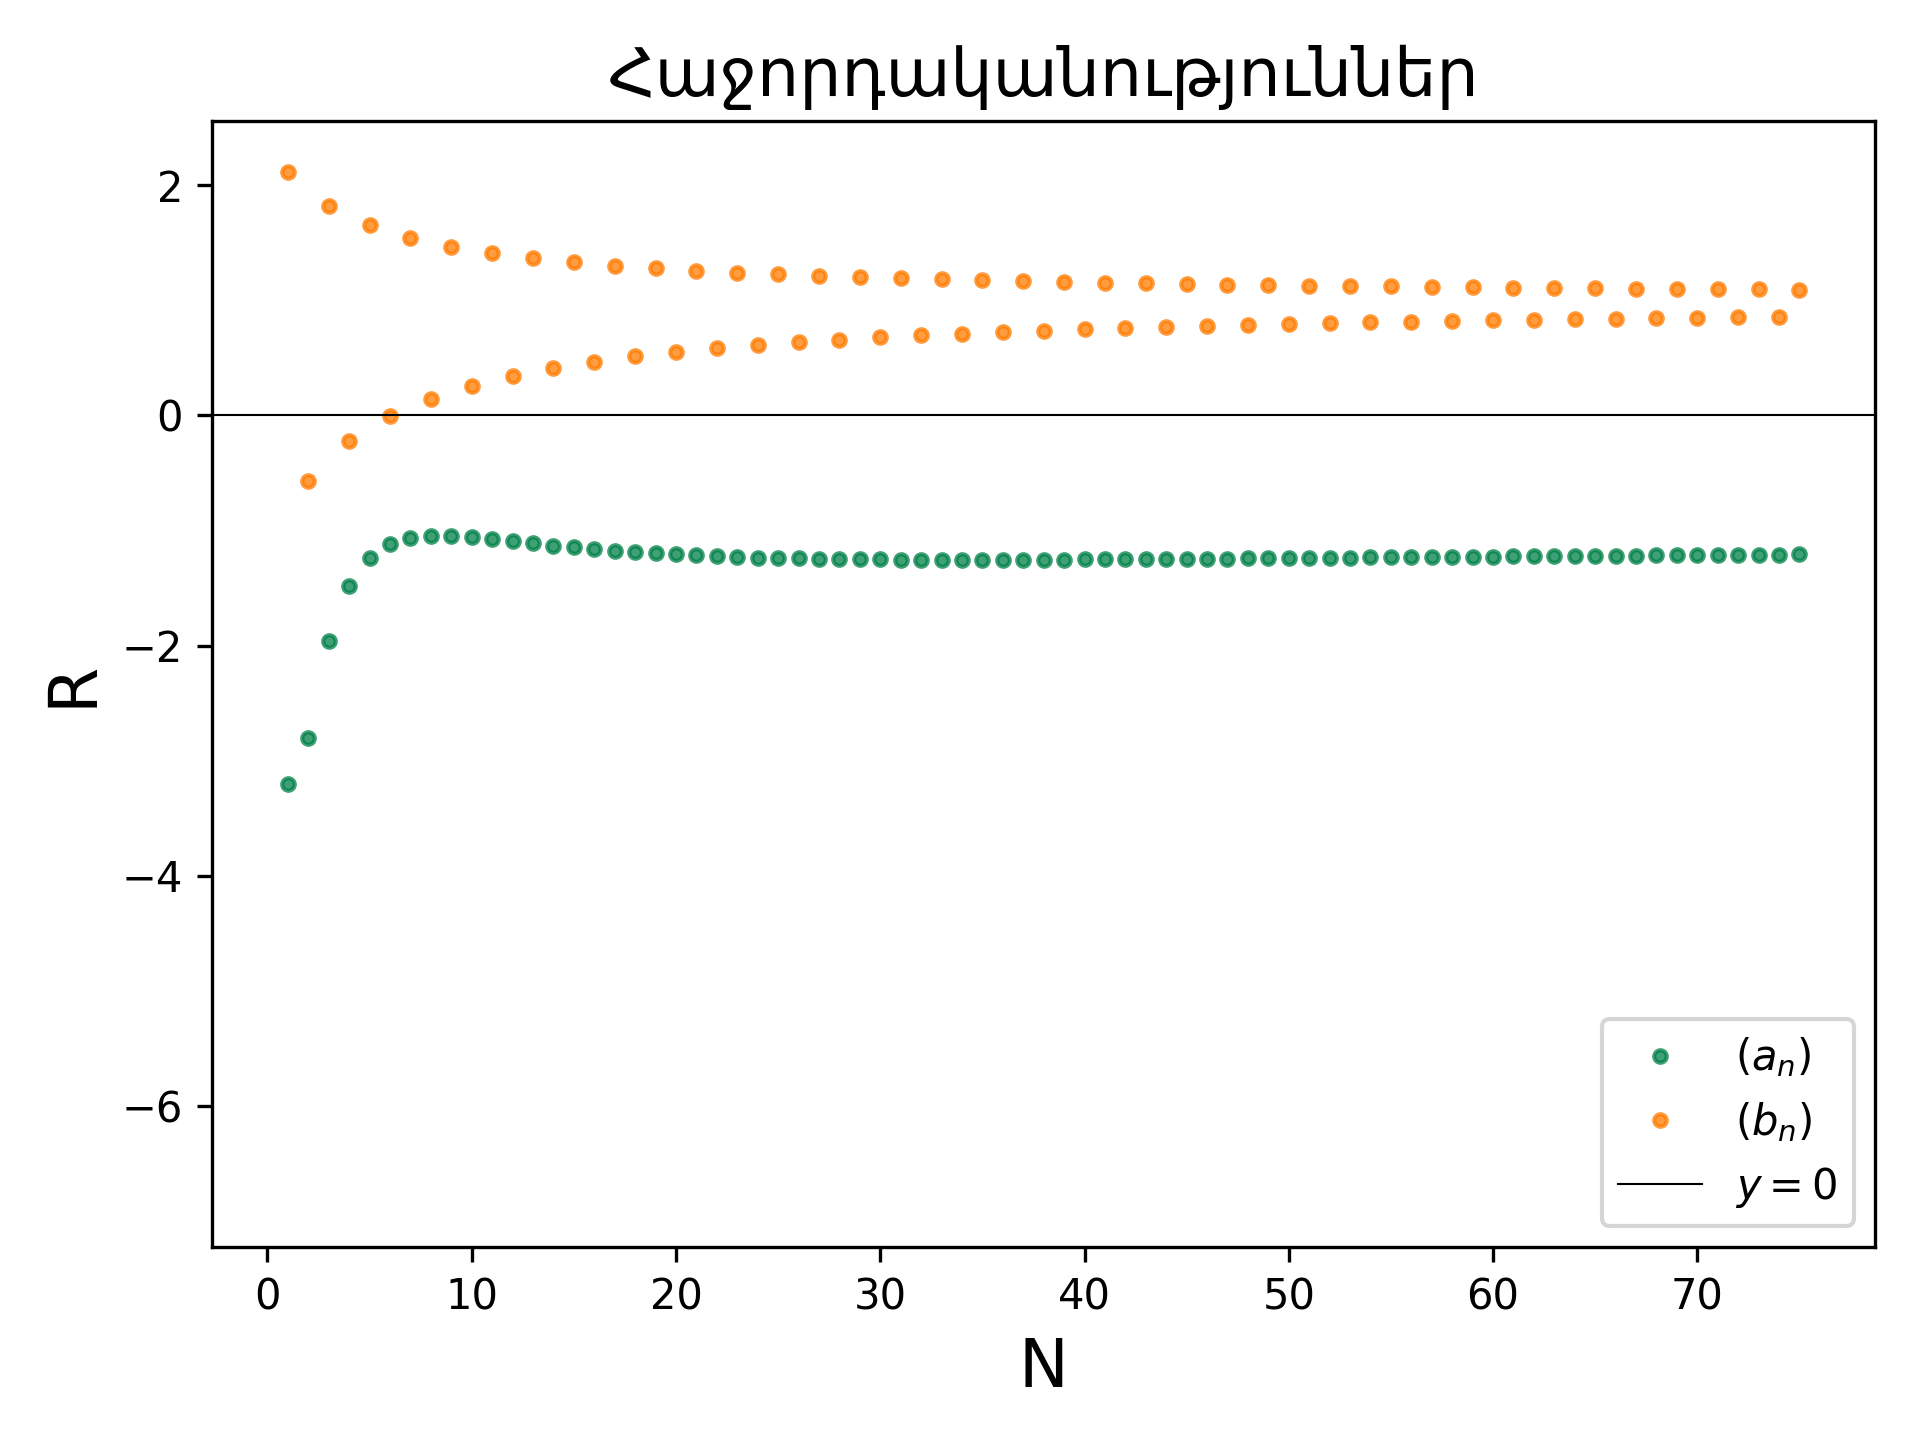
\includegraphics[width=0.3\textwidth]{sequence_poly_plot_.png}}
                \only<3->{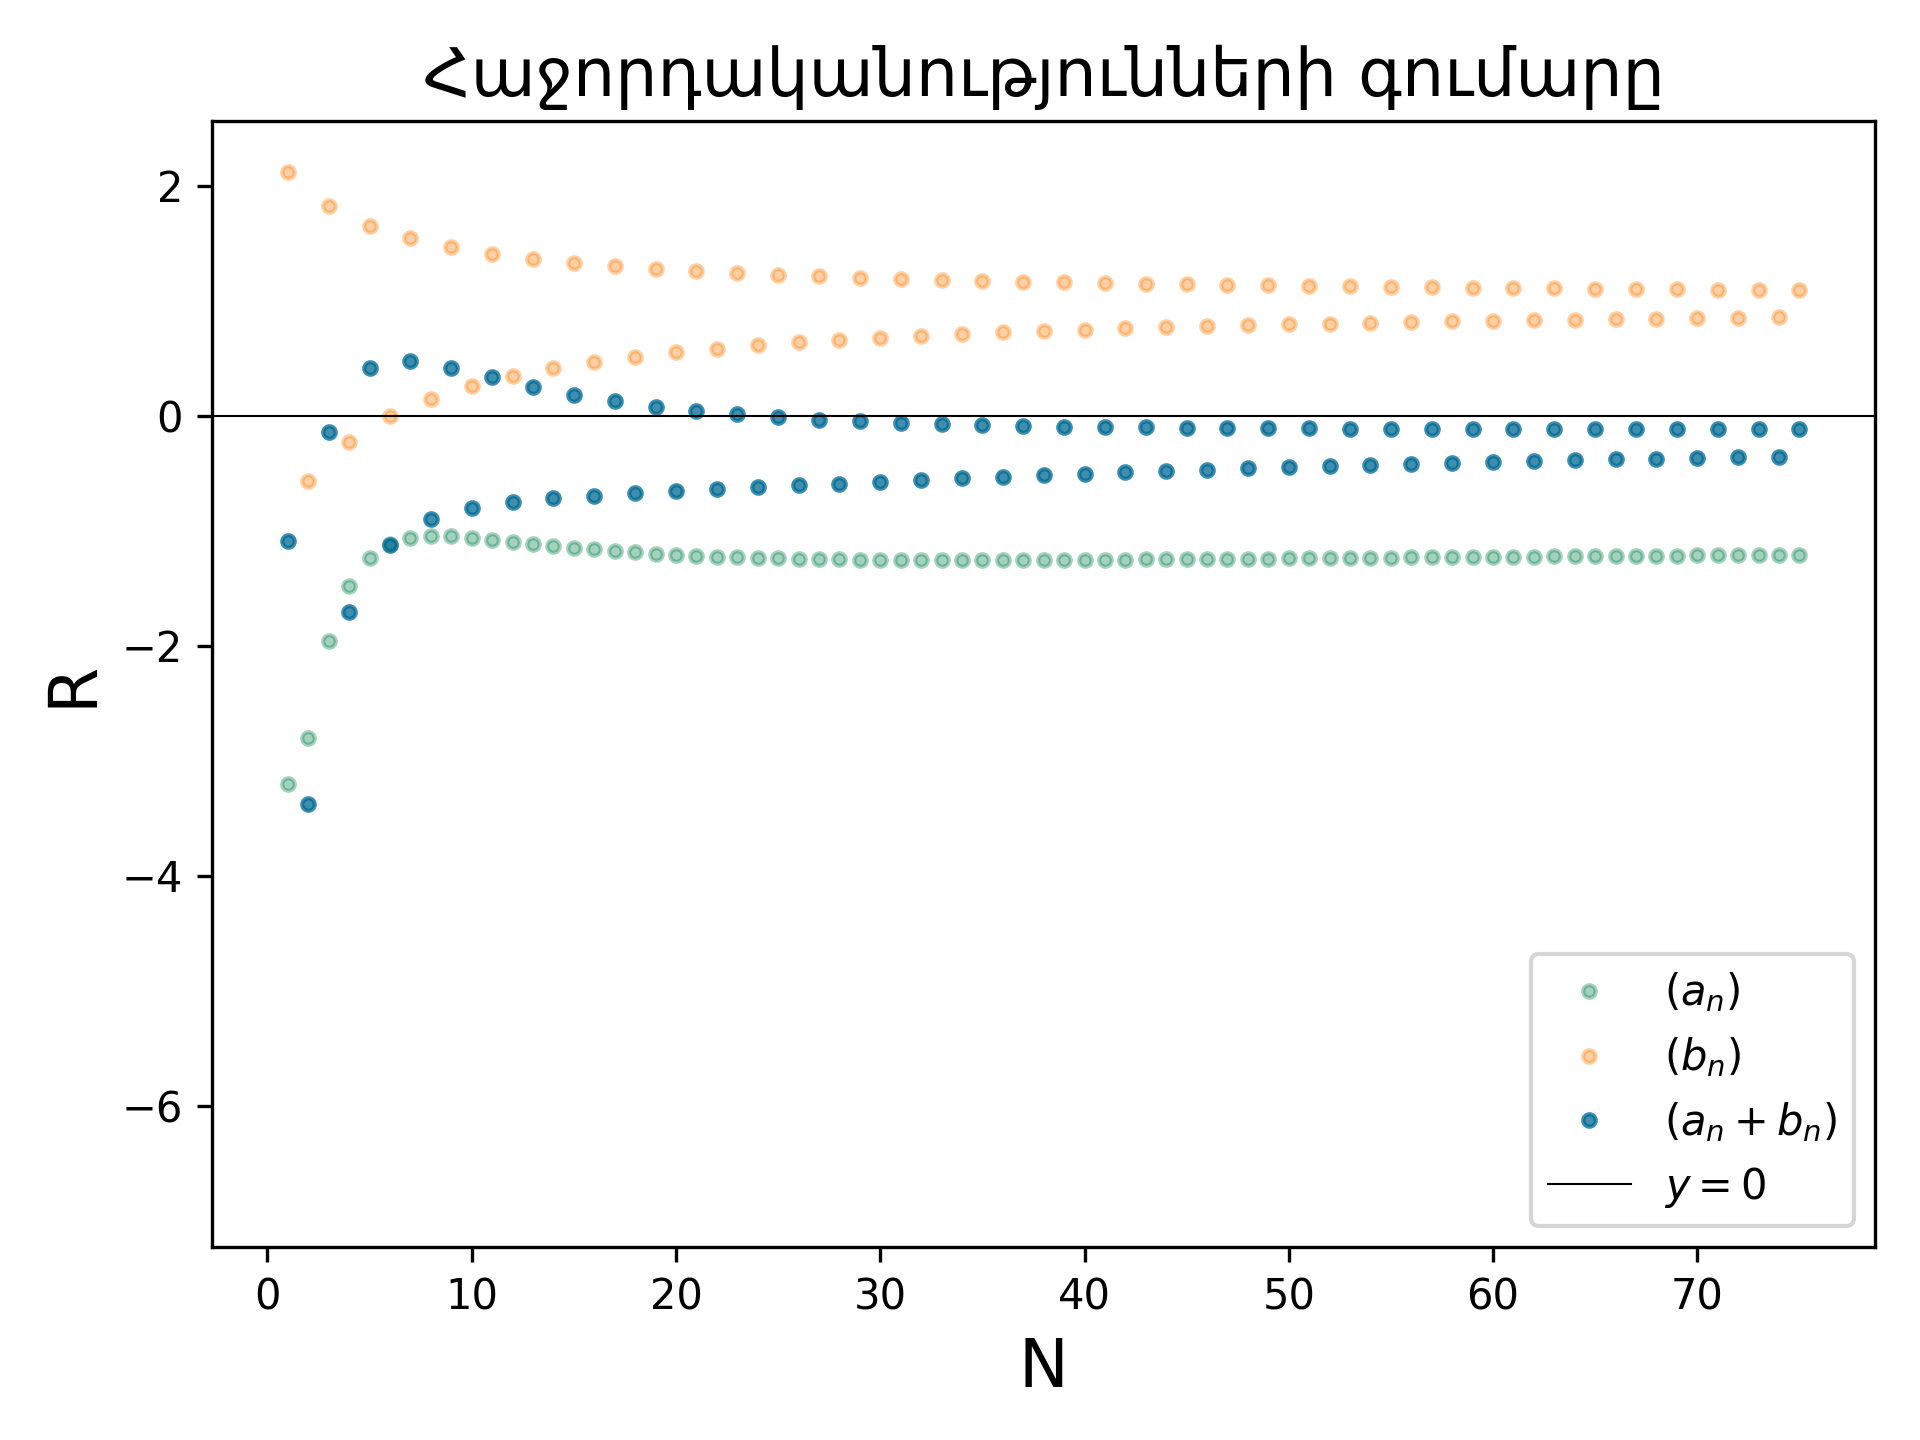
\includegraphics[width=0.3\textwidth]{sequence_poly_plot_sum.png}}
                \only<4->{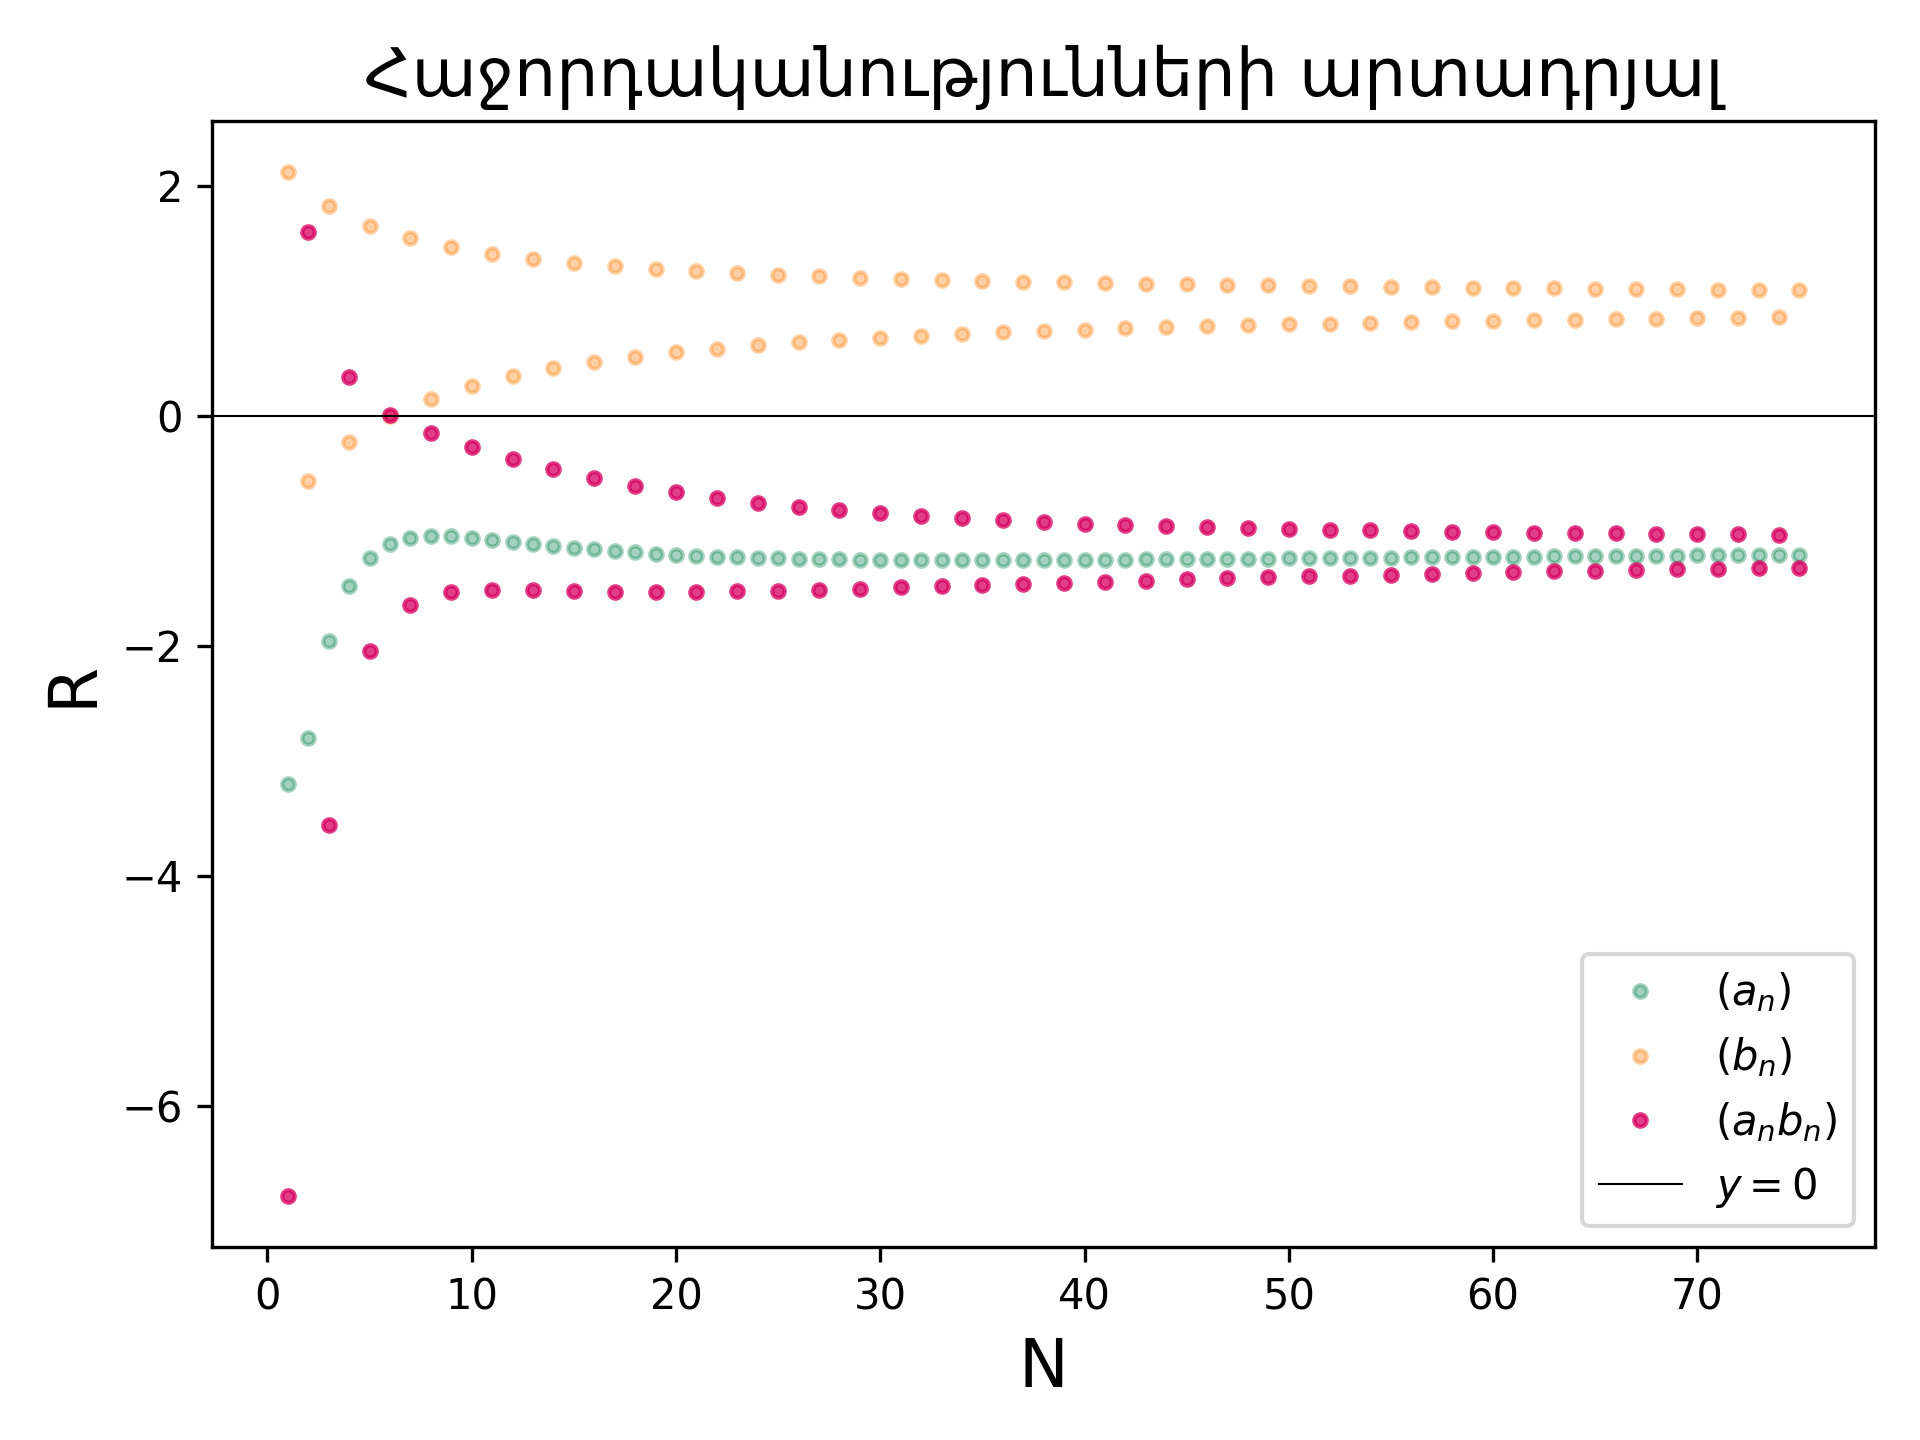
\includegraphics[width=0.3\textwidth]{sequence_poly_plot_mul.png}}
                \only<5>{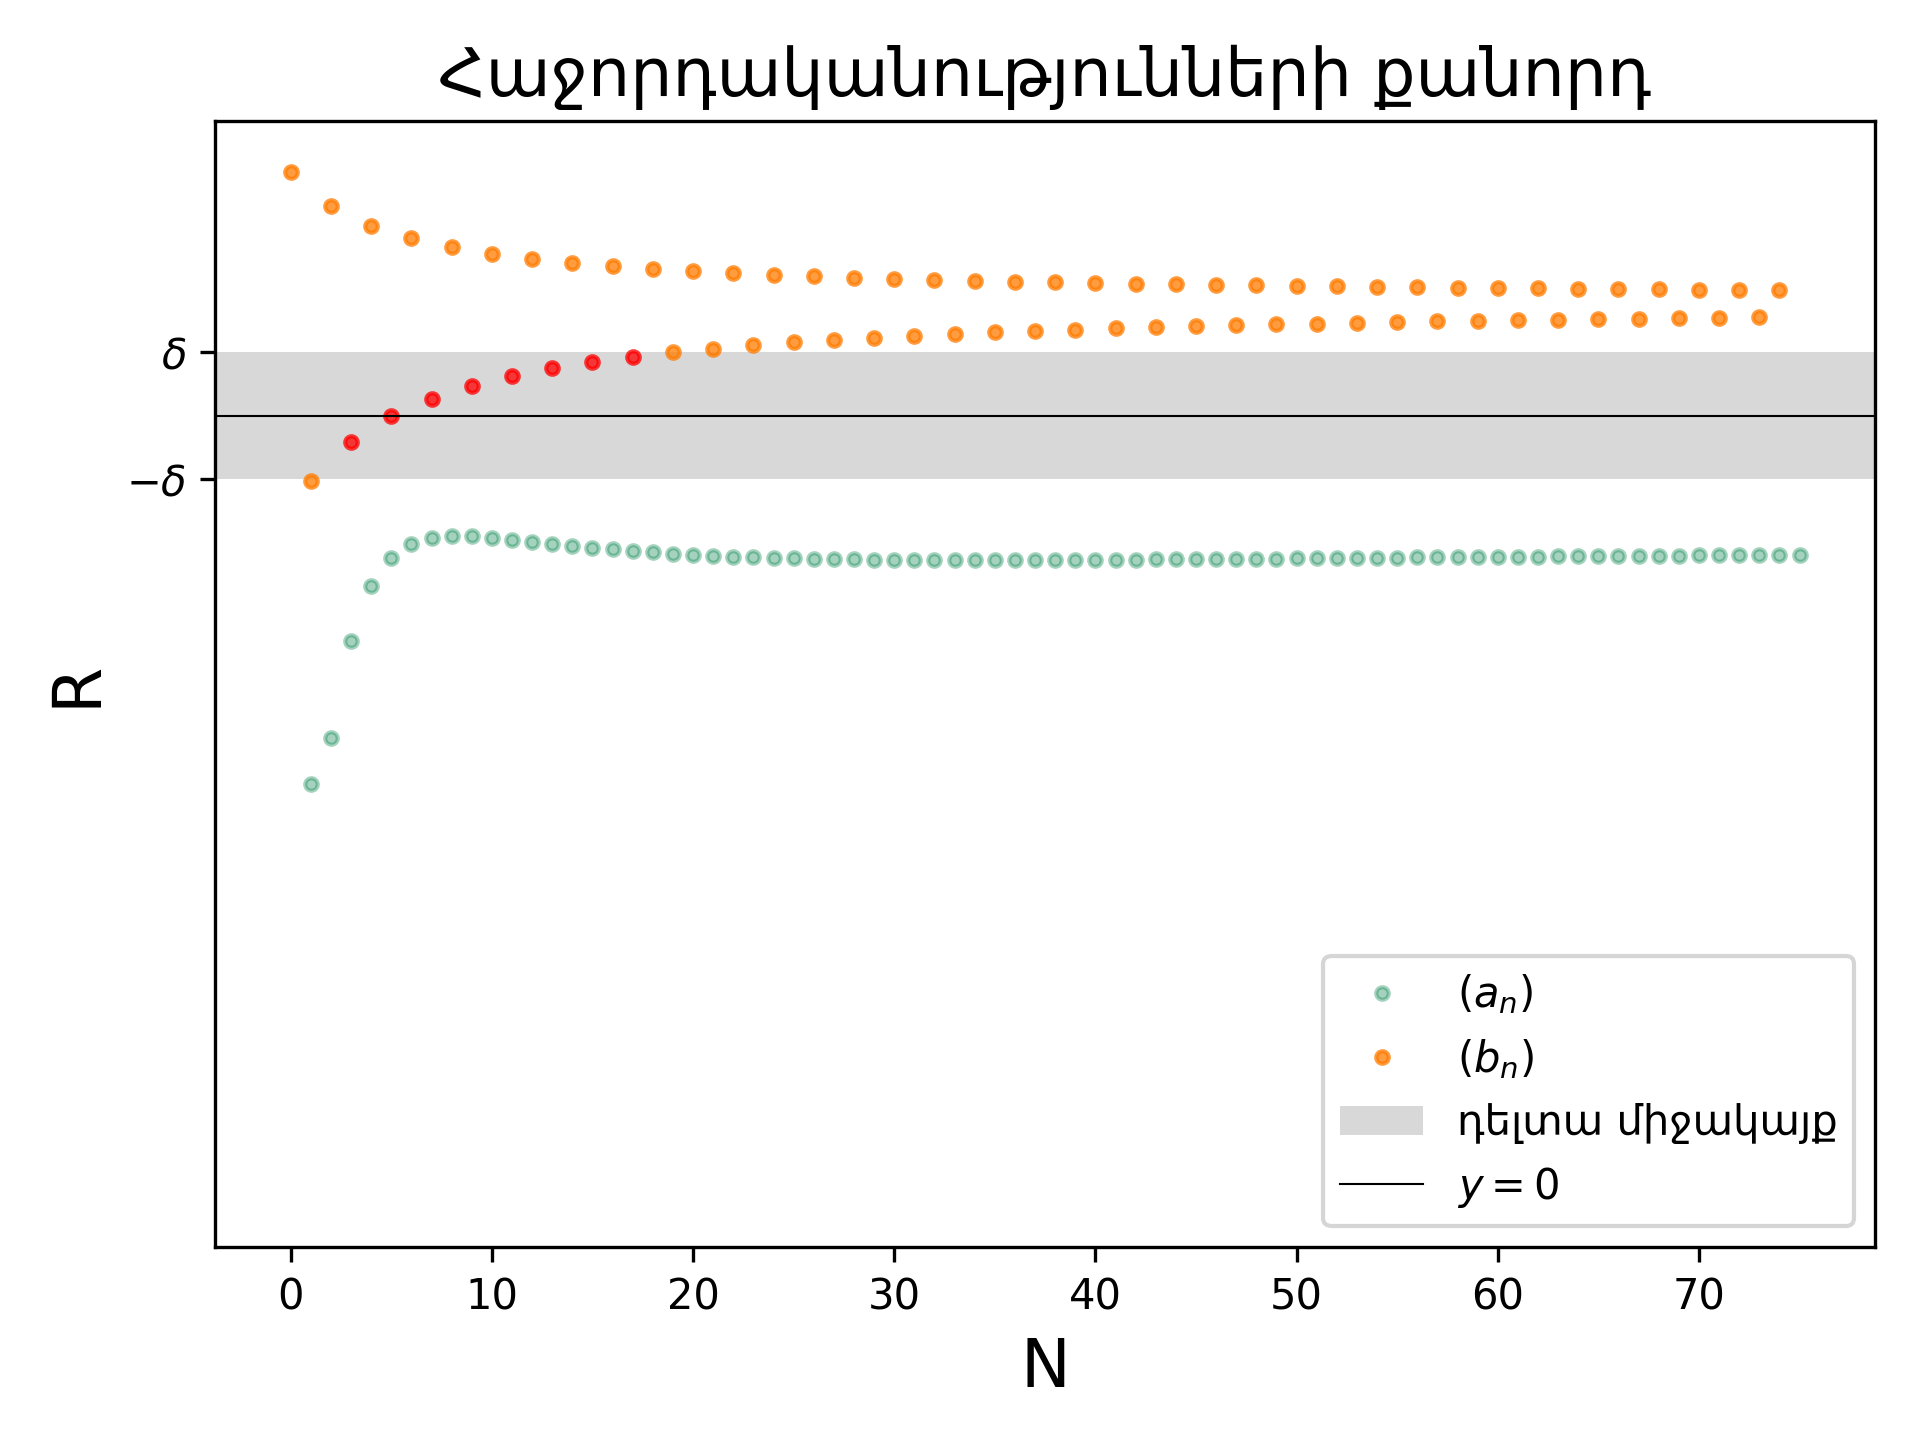
\includegraphics[width=0.3\textwidth]{sequence_poly_plot_frac.png}}
                \only<6>{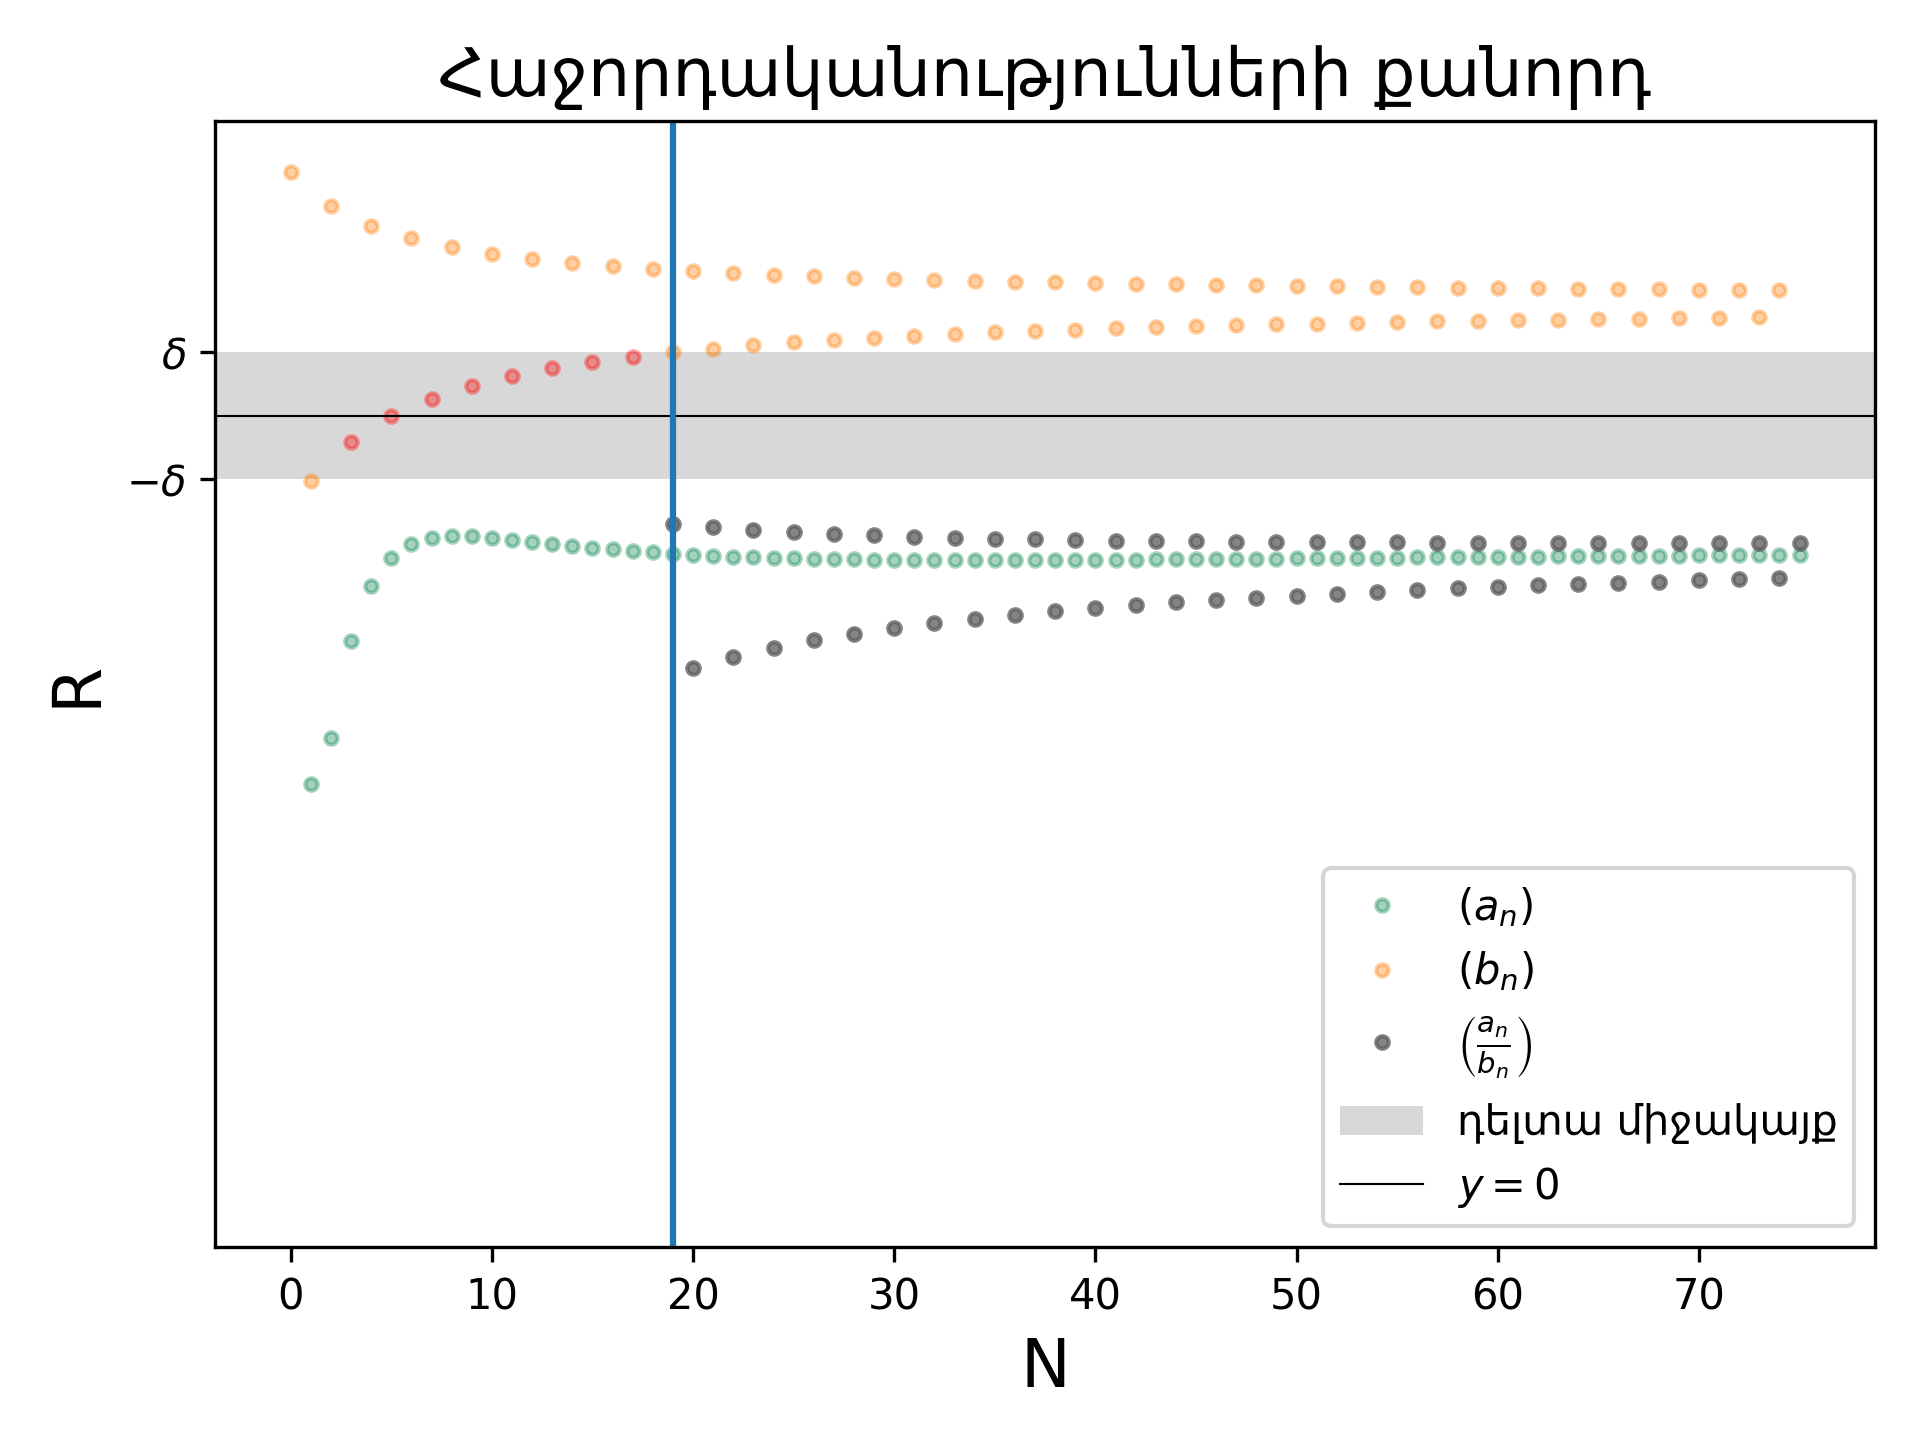
\includegraphics[width=0.3\textwidth]{sequence_poly_plot_frac_2v_l.png}}
            }
        }
    \end{frame}
	\begin{frame}
        \frametitle{Ֆունդամենտալ հաջորդականություն}
        \framesubtitle{Գումար}
        Դիցուք $(a_n)$ և $(b_n)$ հաջորդականությունները ֆունդամենտալ են։
        \begin{block}{Պնդում}
            $(c_n)$ հաջորդականությունը ֆունդամետալ է, որտեղ $c_n = a_n + b_n:$
        \end{block}
        \only<2->{
            \begin{alertblock}{Ապացույց}
                \only<2-> {Ունենք, որ}
                \only<3-> {կամայական տրված $\varepsilon$ դրական թվի համար, սկսած ինչ֊որ պահից \textcolor<7>{red}{$|a_n - a_m| < \varepsilon$} և \textcolor<7>{red}{$|b_n - b_m| < \varepsilon$}։\\}
                \only<4-> {Պետք է գնահատաենք $|c_n - c_m|$֊ը։\\}
                \only<5> {$|c_n - c_m| = |(a_n + b_n) - (a_m + b_m)|$}
                \only<6> {$|c_n - c_m| = |(a_n + b_n) - (a_m + b_m)| = |(a_n - a_m) + (b_n - b_m)|$}
                \only<7-> {$|c_n - c_m| = |(a_n + b_n) - (a_m + b_m)| = |\underbrace{(a_n - a_m)}_{\textcolor<7>{red}{\in (-\varepsilon, \varepsilon)}} + \underbrace{(b_n - b_m)}_{\textcolor<7>{red}{\in (-\varepsilon, \varepsilon)}}|$}
                \only<8-> {$< 4 \varepsilon$}
            \end{alertblock}
        }
    \end{frame}
    \begin{frame}
        \frametitle{Ֆունդմաենտալ հաջորդականություն}
        \framesubtitle{Քանորդ}
        Դիցուք $(a_n)$ և $(b_n)$ հաջորդականությունները ֆունդամենտալ են, ընդորում սկսած ինչ֊որ պահից $|b_n|> \delta > 0:$
        \begin{block}{Պնդում}
            $(c_n)$ հաջորդականությունը ֆունդամետալ է, որտեղ \textcolor<6>{red}{$c_n = \frac{a_n}{b_n}$:}
        \end{block}
        \only<2->{
            \begin{alertblock}{Ապացույց}
                \only<2-> {Ունենք, որ}
                \only<3-> {կամայական տրված $\varepsilon$ դրական թվի համար, սկսած ինչ֊որ պահից \alert<12>{$|a_n - a_m| < \varepsilon$} և \alert<12>{$|b_n - b_m| < \varepsilon$}։\\}
                \only<4-> {Նայև ունենք, որ ինչ֊որ պահից \textcolor<8>{red}{$|b_n| > \delta > 0$}:\\}
                \only<5-> {Պետք է գնահատաենք $|c_n - c_m|$֊ը։\\}
                \only<6> {$|c_n - c_m| = \left|\frac{a_n}{b_n} - \frac{a_m}{b_m}\right|$}
                \only<7> {$|c_n - c_m| = \left|\frac{a_n}{b_n} - \frac{a_m}{b_m}\right| = \left|\frac{a_n b_m - a_m b_n}{b_n b_m}\right|$}
                \only<8> {$|c_n - c_m| = \left|\frac{a_n}{b_n} - \frac{a_m}{b_m}\right| = \left|\frac{a_n b_m - a_m b_n}{b_n b_m}\right| < \textcolor{red}{\frac{1}{\delta^2}}|a_n b_m - a_m b_n|$}
                \only<9> {$|c_n - c_m| = \left|\frac{a_n}{b_n} - \frac{a_m}{b_m}\right| = \left|\frac{a_n b_m - a_m b_n}{b_n b_m}\right| < \frac{1}{\delta^2}|a_n b_m - a_m b_n + \underbrace{(a_nb_n - a_nb_n)}_{=0}|$}
                \only<10> {$|c_n - c_m| = \left|\frac{a_n}{b_n} - \frac{a_m}{b_m}\right| = \left|\frac{a_n b_m - a_m b_n}{b_n b_m}\right| < \frac{1}{\delta^2}|a_n b_m \underbrace{- a_nb_n + a_nb_n}_{=0} - a_m b_n|$}
                \only<11> {$|c_n - c_m| = \left|\frac{a_n}{b_n} - \frac{a_m}{b_m}\right| = \left|\frac{a_n b_m - a_m b_n}{b_n b_m}\right| < \frac{1}{\delta^2}|a_n(b_m - b_n) + b_n(a_n - a_m)|$}
                \only<12> {$|c_n - c_m| = \left|\frac{a_n}{b_n} - \frac{a_m}{b_m}\right| = \left|\frac{a_n b_m - a_m b_n}{b_n b_m}\right| < \frac{1}{\delta^2}|a_n\alert{\underbrace{(b_m - b_n)}_{\in (-\varepsilon, \varepsilon)}} + b_n\alert{\underbrace{(a_n - a_m)}_{\in (-\varepsilon, \varepsilon)}}|$}
                \only<13> {$|c_n - c_m| = \left|\frac{a_n}{b_n} - \frac{a_m}{b_m}\right| = \left|\frac{a_n b_m - a_m b_n}{b_n b_m}\right| < \frac{1}{\delta^2}|\alert{\underbrace{a_n}_{\in [-M, M]}}(b_m - b_n) + \alert{\underbrace{b_n}_{\in [-M, M]}}(a_n - a_m)|$}
                \only<14> {$|c_n - c_m| = \left|\frac{a_n}{b_n} - \frac{a_m}{b_m}\right| = \left|\frac{a_n b_m - a_m b_n}{b_n b_m}\right| < \frac{1}{\delta^2}|a_n(b_m - b_n) + b_n(a_n - a_m)| \le \frac{2M}{\delta^2} \varepsilon $}
                
                % \only<13> {$|c_n - c_m| = \left|\frac{a_n}{b_n} - \frac{a_m}{b_m}\right| = \left|\frac{a_n b_m - a_m b_n}{b_n b_m}\right| < \frac{1}{\delta^2}|\underbrace{(a_n - a_m)}_{\in (-\varepsilon, \varepsilon)}(b_m + b_n)  - a_n(b_n - b_m)(b_n - b_m)|$}
                % \only<13> {$|c_n - c_m| = \left|\frac{a_n}{b_n} - \frac{a_m}{b_m}\right| = \left|\frac{a_n b_m - a_m b_n}{b_n b_m}\right| < \frac{1}{\delta^2}|\underbrace{(a_n - a_m)}_{\textcolor<13>{red}{\in (-\varepsilon, \varepsilon)}}(b_m + b_n)|$}
                % \only<14> {$|c_n - c_m| = \left|\frac{a_n}{b_n} - \frac{a_m}{b_m}\right| = \left|\frac{a_n b_m - a_m b_n}{b_n b_m}\right| < \frac{1}{\delta^2}|\underbrace{(a_n - a_m)}_{\textcolor<13>{red}{\in (-\varepsilon, \varepsilon)}}\underbrace{(b_m + b_n)}_{\textcolor<14>{red}{\leq 2M  \text{ $(b_n)$-ը սհամանափակ է}}}|$}
                % \only<15> {$|c_n - c_m| = \left|\frac{a_n}{b_n} - \frac{a_m}{b_m}\right| = \left|\frac{a_n b_m - a_m b_n}{b_n b_m}\right| < \frac{1}{\delta^2}|\underbrace{(a_n - a_m)}_{\textcolor<13>{red}{\in (-\varepsilon, \varepsilon)}}\underbrace{(b_m + b_n)}_{\textcolor<14>{red}{\leq 2M}}| \le \frac{2M}{\delta^2} \varepsilon$}
            \end{alertblock}
        }
   \end{frame}
\end{document}